\chapter{Computational study}
\label{chap:computational_study}
This chapter will give the most insights into the functionality and efficiency of the usage of the presented binary classifier in
\gls{3L-CVRP} algorithms. This chapter will begin with the selection of two published \gls{3L-CVRP} datasets.
Afterwards, the results from the model training are presented, which
is divided in three main parts, firstly the results of the retrieval of the data, secondly the feature selection, and finally presenting
different strategies for comparing different models and selecting the best best fit performance wise.
Thereafter, a parameter study is conducted for the \gls{ILS}, starting with the NoClassifier variant determining
the best configurations for the base parameters, followed by a variant specific parameter study.
This chapter closes with a computational study of all four variants, comparing the variants with tuned parameters.
The insights are summarized in the concluding chapter. All experiments were run on a AMD EPYC 7513 32-Core machine
with 8 cores maximum available for the \gls{CP} solver. The \gls{ILS} algorithm is implemented in C++ and all models
were pretrained in Python and loaded afterwards in the metaheuristic. All data analysis was carried out in either Python scripts
or Jupyter notebooks. The Section~\ref{app:sec:github_implementations} in the appendix contains the links to all GitHub repositories of the implementations.

\section{Comparison of Available Datasets}
\label{sec:dataset_comparison}

The \gls{3L-CVRP} is a well-studied problem and several datasets were published in the past, considering
different constraints and characteristics. A selection of these datasets will be compared and evaluated
in this section. The goal is to identify suitable datasets for training a general \gls{CLP} classifier that can predict
the loading feasibility of single tours from different datasets. Therefore, the dataset needs
heterogeneous characterists to represent numerous possible use-cases
as shown in Section~\ref{sec:motivation_feasibility_prediction}. Five published
\cgls{3L-CVRP} datasets are presented with respect to their overall characteristics.
Each dataset gets an unique identfier to simplify the comparison and is shown in parenthesis
after the following individual introduction. The first \cgls{3L-CVRP} dataset was published by \citeauthor{gendreau_tabu_2006} in
\citeyear{gendreau_tabu_2006} and delivered instances containing huge and heavy items (\gendreauDataSet).\footcite[cf.][]{gendreau_tabu_2006}
The second dataset was published by \citeauthor{moura_integrated_2009} in \citeyear{moura_integrated_2009},
and combines the \gls{VRP} from \citeauthor{solomon_algorithms_1987} and the \gls{CLP} instances from
\citeauthor{bischoff_issues_1995} defining the \gls{3L-VRPTW} considering
many items of small size and weight (\mouraDataSet).\footcites[cf.][]{solomon_algorithms_1987}[][]{bischoff_issues_1995}[][]{moura_integrated_2009}
The first dataset containing real-life data was published by \citeauthor{ceschia_local_2013} in \citeyear{ceschia_local_2013}
and contains the instances with the most items (\ceschiaDataSet).\footcite[cf.][]{ceschia_local_2013}
Krebs published two different datasets in
\citeyear{krebs_advanced_2021} with a focus on more realistic constraints. The first one contains a set
of realistic constraints and offers a wide range of instance sizes (\krebsADataSet).\footcite[cf.][]{krebs_advanced_2021}
The second one focuses on semi-trailer trucks and special requirements for axle weights (\krebsBDataSet).\footcite[cf.][]{krebs_axle_2021}
The characteristics of the datasets are summarized in the following Table~\ref{tab:dataset_comparison},
where the brackets [\,] indicate a range of possible values. All values considering mass and volume are
\textit{relative} to the respective vehicle weight and volume limit to be comparable. A \textit{item type} is
defined by its geometrical dimensions, the weight, and possible stability characteristics, such as fragility or \gls{LBS}.
The types column depict the number of different item types per instance.
When the number of item types is smaller than the number of items, equal item types occur multiple times. Additionally,
most features of the dataset are compared with \textit{aggregated}  values, referring to the aggregrated characteristics
of all items requested by one customer, so the aggregated mass, volume and items shows the average value requested by an
customer of this dataset.

\newcolumntype{C}[1]{>{\centering\arraybackslash}p{#1}}
\newcolumntype{L}[1]{>{\raggedright\arraybackslash}p{#1}} % left-aligned
\begin{table}[ht]
    \centering
    \small
    \renewcommand{\arraystretch}{1.1}   % a touch more row height
    \begin{tabular}{@{}lccccc@{}}
        \toprule
        \textbf{Dataset} & \textbf{Instances} & \textbf{Customers} & \textbf{Agg. Mass}\footnote{Average is based on all customers of the instances.} & \textbf{Agg. Vol.} \footnotemark[\value{footnote}]       & \textbf{Agg. Items}\footnotemark[\value{footnote}] \\
        \midrule
        \gendreauDataSet & 27                 & [15, 100]          & 0.137                                                                            & 0.127                                                    & 2.00                                               \\
        \mouraDataSet    & 46                 & 25                 & 0.077                                                                            & 0.176                                                    & 52.0                                               \\
        \ceschiaDataSet  & 13                 & [11, 129]          & 0.063                                                                            & 0.160                                                    & 18.1                                               \\
        \krebsADataSet   & 600                & [20, 100]          & 0.098                                                                            & 0.100                                                    & 4.41                                               \\
        \krebsBDataSet   & 80                 & [30, 120]          & 0.036                                                                            & 0.052                                                    & 4.00                                               \\
        \toprule
        \textbf{Dataset} & \textbf{Items}     & \textbf{Types}     & \textbf{\text{Routes}}\footnote{Average is based on the instances.}              & \textbf{\text{Route Len}}\footnotemark[\value{footnote}] & \textbf{Fragility}\footnotemark[\value{footnote}]  \\
        \midrule
        \gendreauDataSet & [26, 199]          & [26, 199]          & 6.13                                                                             & 6.22                                                     & 0.25                                               \\
        \mouraDataSet    & 1050, 1550         & 5                  & 4.40                                                                             & 6.72                                                     & 0.29                                               \\
        \ceschiaDataSet  & [254, 8060]        & [9, 97]            & 10.2                                                                             & 5.81                                                     & 0.10                                               \\
        \krebsADataSet   & 200, 400           & 3, 10, 100         & 6.77                                                                             & 13.6                                                     & 0.24                                               \\
        \krebsBDataSet   & 200, 400           & 10, 100            & 3.87                                                                             & 22.1                                                     & 0.10                                               \\
        \bottomrule
    \end{tabular}
    \caption[Numerical comparison of different 3L--CVRP Datasets.]{Numeric comparisons between five avalaible datasets.}
    \label{tab:dataset_comparison}
\end{table}

The columns routes, route length and fragility show the average over all instances.
Routes define the \gls{LB} for the needed vehicles $K$ and route length the average number of customers per route based
on the relative volume and mass. The averages are displayed to become a better understanding of the
statistics of each dataset, rather than looking at extreme values.
The most important consideration, when selecting a suitable dataset for the training of a classifier,
is how representative single tours from one dataset are for all other datasets. Therefore, the numeric characteristics
should not contain outliers. It is apparent, that the \gendreauDataSetText dataset has the least items per customer
with huge relative volume and weight, which leads with an average route length of 6.22 customers to very few items
considered per route in comparison to the other datasets. This makes it easier to compute the feasibility of the loading
as the combinations of placing patterns is limited. The \mouraDataSetText dataset has the most items per average per customer consisting
of only 5 item types. The \ceschiaDataSetText dataset contains the fewest instances, but with the most items of 8060,
which lead to many routes on average. The two datasets from Krebs, have similar
boundaries and values, but \krebsBDataSetText has routes with twice as many customers as \krebsADataSetText on average due
to the smaller average aggregated mass and volume. Both \krebsADataSetText and \gendreauDataSetText,
show a good variety of the features, without including too many items per route in comparison to the other datasets.
However, as the average route length from \krebsADataSetText is twice as long and the number of items per customer contain twicw as many,
one route contain per average four times more items leading to a higher complexity for solving the \gls{CLP}.
The following Table~\ref{tab:constraint_matrix} provides an overview of the constraints considered
in each dataset showcasing the realistic profile. The constraints are categorized into the five loading constraint groups introduced
in Section~\ref{sec:clp_definition}.
\clearpage

\begin{table}[ht]
    \centering
    \small
    \renewcommand{\arraystretch}{1.2}
    \begin{tabular}{@{}L{1.8cm}L{3cm}C{1.6cm}C{1.6cm}C{1.6cm}C{1.6cm}C{1.6cm}@{}}
        \toprule
        \textbf{Category}          & \textbf{Constraint} &                        &                     & \textbf{Dataset}      &                      &                      \\
                                   &                     & Gendreau\newline(2006) & Moura\newline(2009) & Ceschia\newline(2013) & Krebs\newline(2021a) & Krebs\newline(2021b) \\
        \midrule
        \multirow{3}{*}{Container} & Load Capacity       & $\bullet$              & $\bullet$           & $\bullet$             & $\bullet$            & $\bullet$            \\
                                   & Load Balance        &                        &                     &                       & $\bullet$            &                      \\
                                   & Axle Weights        &                        &                     &                       & $\bullet$            & $\bullet$            \\\midrule
        \multirow{3}{*}{Item}      & z-Rotation          & $\bullet$              & $\bullet$           & $\bullet$             & $\bullet$            & $\bullet$            \\
                                   & Fragility           & $\bullet$              &                     & $\bullet$             & $\bullet$            & $\bullet$            \\
                                   & LBS                 &                        &                     & $\bullet$             & $\bullet$            &                      \\\midrule
        \multirow{1}{*}{Cargo}     & Complete Shipm.     & $\bullet$              & $\bullet$           &                       & $\bullet$            & $\bullet$            \\\midrule
        \multirow{6}{*}{Position}  & Geometry            & $\bullet$              & $\bullet$           & $\bullet$             & $\bullet$            & $\bullet$            \\
                                   & Orthogonality       & $\bullet$              & $\bullet$           & $\bullet$             & $\bullet$            & $\bullet$            \\
                                   & Reachability        &                        &                     & $\bullet$             & $\bullet$            &                      \\
                                   & Sequence            & $\bullet$              &                     &                       & $\bullet$            &                      \\
                                   & LIFO                & $\bullet$              & $\bullet$           & $\bullet$             & $\bullet$            & $\bullet$            \\
                                   & MLIFO               &                        &                     & $\bullet$             & $\bullet$            &                      \\\midrule
        \multirow{2}{*}{Load}      & Robust Stability    &                        &                     & $\bullet$             & $\bullet$            &                      \\
                                   & Support Area        & $\bullet$              & $\bullet$           &                       &                      & $\bullet$            \\

        \bottomrule
    \end{tabular}
    \caption[Overview of CLP constraints in selected 3L--CVRP datasets.]{Matrix overview of constraints covered in selected datasets. A bullet ($\bullet$) indicates that the constraint is considered.}
    \label{tab:constraint_matrix}
\end{table}

This comparison shows, that all datasets include similar types of constraints, but the level
of complexity varies. \krebsADataSetText and \ceschiaDataSetText stand out by incorporating
more advanced constraints such as robust stability, reachability, and \gls{LBS}, in comparison to
basic ones like support area, \gls{LIFO} and fragility. To further investigate the differences
between the datasets, Figure~\ref{fig:dataset_comparison} visualizes the aggregated relative mass and
volume of all items requested by individual customers.
Additionally, the size of each scatter point indicates the total number of items requested.
For example, the \mouraDataSetText dataset includes 46
instances with 25 customers each, resulting in $25 \cdot 46 = 1150$ dots in the plot.

\begin{figure}[ht]
	\centering
	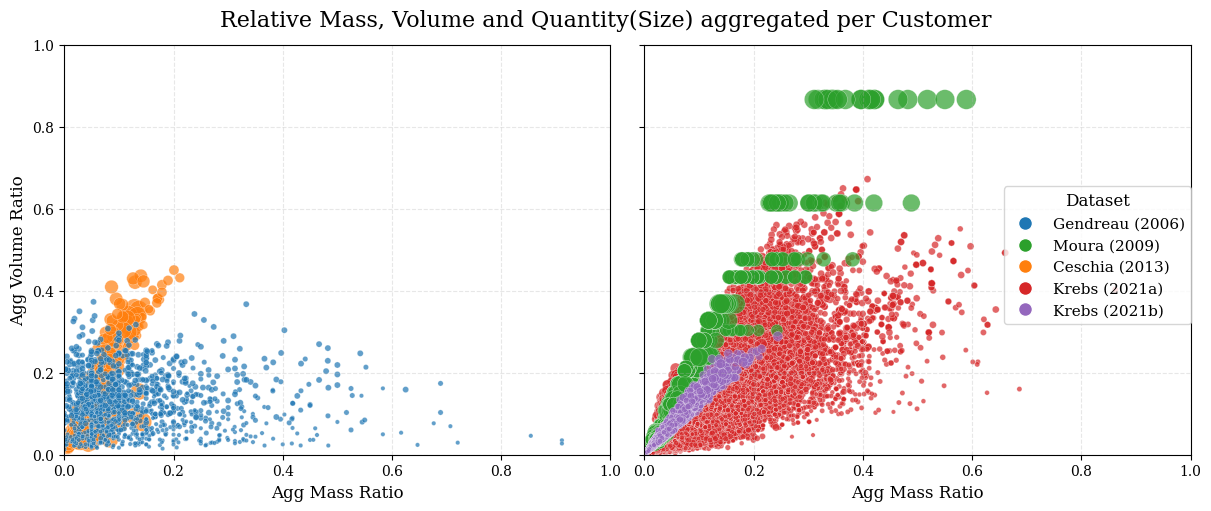
\includegraphics[width=0.85\textwidth]{pictures/comparison_datasets_3lcvrp.png}
	\caption{Comparison aggregated customer demands of different vehicle routing problem datasets with loading constraints.}
	\label{fig:dataset_comparison}
\end{figure}

The dispersion of the data points reflects the diversity of individual instances in terms of volume
and mass dependency. A more balanced profile suggests that some customers tend to order items that
are either mass- or volume-intensive, which supports training the model on more heterogeneous data.
Therefore, the dataset should cover a wide range of cases, varying in mass, volume, and item
quantity per customer. The widest spread is observed in \krebsADataSetText and \gendreauDataSetText serving
both as good dataset candidates for training a classifier, which are analyzed further in
the next section.

\section{Analsis of datasets}
\label{sec:analysis_datasets}

The two datasets, \krebsADataSetText and \gendreauDataSet, have a good diverse profile for training
a binary classifier and to be further analyzed.
As shown in Section~\ref{sec:literature_overview} several publications solved the \gendreauDataSetText dataset
with various heuristics and even exact approaches, whereas only one heuristic solution approach exists for the instances of \krebsADataSet.
Both datasets are further analysed in this section to understand dataset specific properties.

\subsubsection{\krebsADataSetText}

The dataset contains 600 instances with 18 instance types derived from the combinations
of number of customers, item types and items. The following Figure~\ref{fig:krebs_dataset_analysis_detailes} plots
the relative mass and volume of all items requested by individual customers for each of the instances. Every color
represents one instance type and the plots are divided by the number of respective customers in three groups, presenting
6 combinations each. There are three levels for the different item types, 3, 10, and 100, and two levels for the total
number of items per instance, namely 200 and 400.
\begin{figure}[ht]
	\centering
	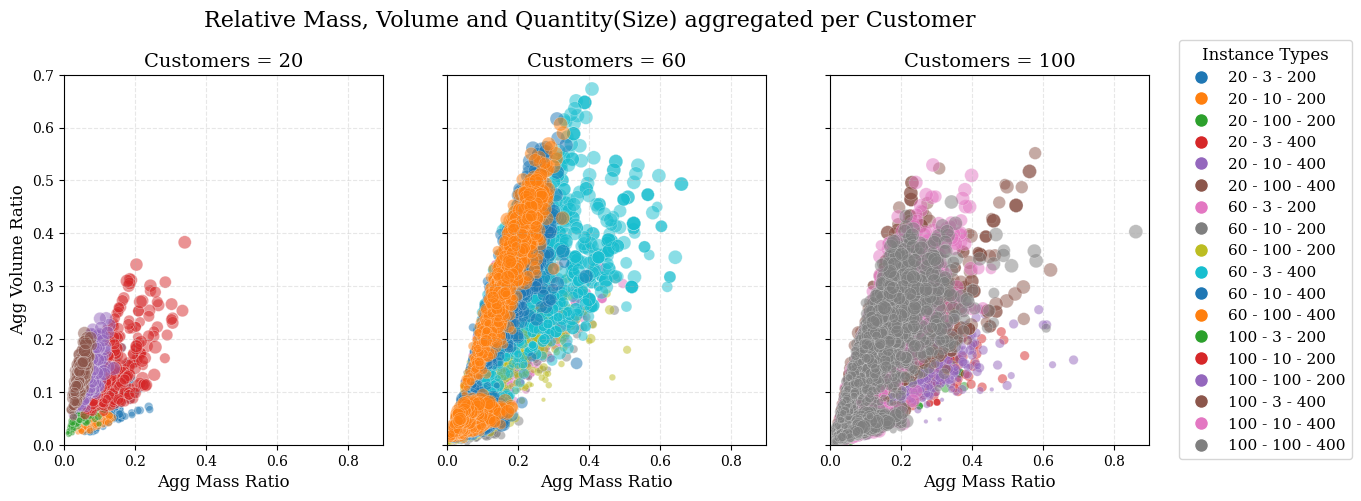
\includegraphics[width=0.85\textwidth]{pictures/krebs_instances_detailed.png}
	\caption[Visualization of different instances of \textcite{krebs_advanced_2021} dataset.]{Visualization of different instances of \krebsADataSetText dataset.
		The instances are named by the number of customers, item types and items.}
	\label{fig:krebs_dataset_analysis_detailes}
\end{figure}%
Several insights can be obtained from the analysis of this plot. Firstly, the aggregated relative
volume and mass per customer is significantly lower for the group with 20 customers than for the groups with 60 or 100 customers.
Secondly, the distribution differs from each instance type, ranging from quite linear distributions in a narrow
interval (e.g. instance 60-100-400) to quite broad distributions (e.g. instance 100-100-400). These two observations need to be considered,
when selecting instances to generate the training data for the classifier to avoid a homogenous training sets.
The instance set should be drawn from every group equally and different distributions need to be considered per group,
that the average numeric route structure differs.

\subsubsection{\gendreauDataSetText}

The dataset consists of 27 instances. The dispersion of the aggregated mass per customer reaches very high values, up to 0.91,
while the corresponding volume levels remain modest, with a maximum of approximately 0.4, as shown in Figure~\ref{fig:dataset_comparison}. The
following Figure~\ref{fig:aggregated_gendreau_plots} show this dispersion per instance revealing an important insight about the dataset.
As the relative volume is quite constant for all instances, the relative mass differs between the instances.
\begin{figure}[ht]
	\centering
	\begin{tikzpicture}[scale=0.9, transform shape,node distance=0mm and 0mm]
		\node[anchor=south, inner sep=0] (A) at (0,0)
		{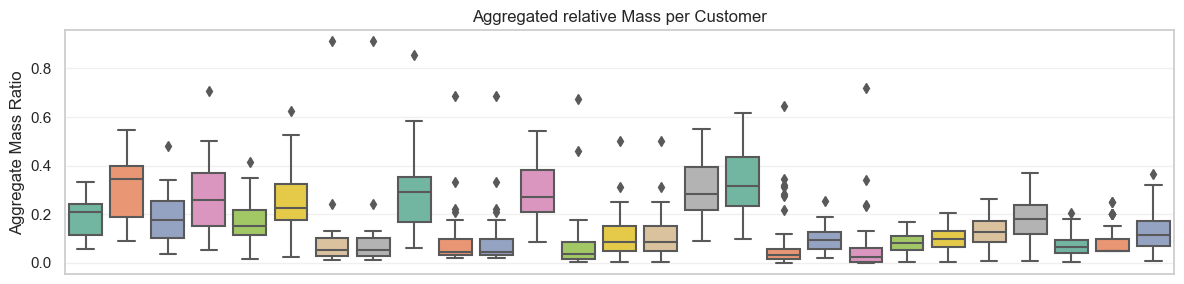
\includegraphics[width=0.95\textwidth]{pictures/AggMassCustGendreau.png}};
		\node[anchor=north, below=of A,inner sep=0] (B)
		{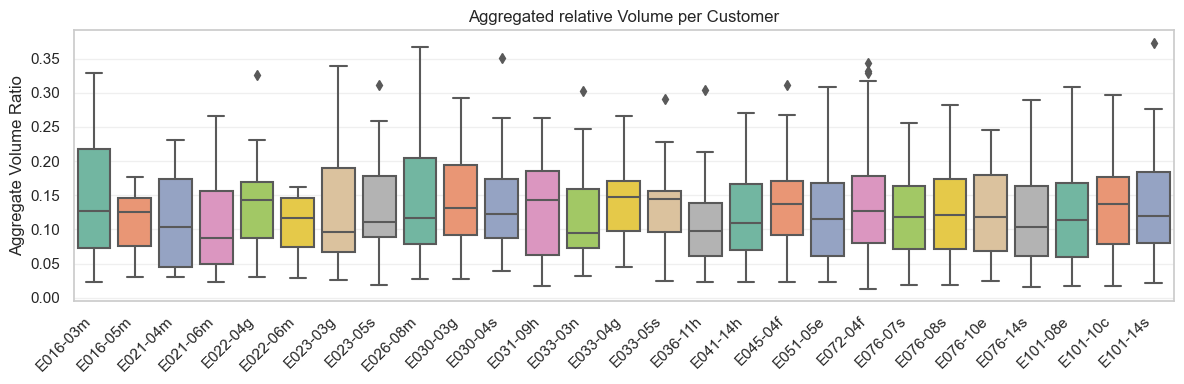
\includegraphics[width=0.96\textwidth]{pictures/AggVolCustGendreau.png}};
	\end{tikzpicture}
	\caption{Aggregated relative mass and volume per customer distributed for each instance of the \gendreauDataSetText dataset.}
	\label{fig:aggregated_gendreau_plots}
\end{figure}
As analyzed in \cite{tamke_branch-and-cut_2024}, the complexity of solving an instance increases significantly when the items are
lightweight and volume, rather than weight, becomes the limiting factor for container loading. The authors further distinguished
the instances into two groups, heavy items ($\mathcal{H}$) and lightweight items ($\mathcal{L}$), based on the average weight
utilization of the final routes obtained.\footcite[cf.][pp. 23--25]{tamke_branch-and-cut_2024}
Since this classification relies on optimal solutions, this thesis adopts an alternative approach to distinguish
both \krebsADataSetText and \gendreauDataSetText into heavyweight (H) and lightweight (L) instances. An instance is classified
as heavyweight, if the mean weight per instance exceeds the overall mean across all instances. This definition has the advantage
that instances lacking optimal solutions can also be labeled.
The obtained results for the \gendreauDataSetText and \krebsADataSetText instances are therefore differentiated into these two groups
to investigate the influence on solution quality and the solution process.

\parbreak

As the construction of train datasets with the \krebsADataSetText dataset is much more computationally challenging than for \gendreauDataSet,
the following sections will focus only on the latter and the Section~\ref{chap:application_krebs} on the \krebsADataSetText dataset.

\section{Feature and Dataset Selection}
\label{sec:ResultsTraining}
In this section the results from the feature and dataset selection are discussed. For each model variant (see Section~\ref{sec:modelselection}),
the most suiting datasets are selected from both, the random and save strategy datasets and
a feature filer algorithm will be discussed. The selected models are used in the computational study to compare the \gls{ILS} algorithm
and its variants.

\subsection{Results Data Retrieval}
\label{subsec:results_retrieval}

\subsubsection{Random Retrieval Strategy}
The following random datasets were generated using Algorithm~\ref{fig:flowchart_randomRouteGeneration},
considering all instances from the \gendreauDataSetText. Notably, the attempts limit parameter ($\beta$) did not have a significant influence
on the number of routes or the dataset structure. Therefore, the datasets with $\beta = 30$ were preselected.
The values in the “Balance” column represent the proportion of positive and negative labels in the sample population.
The relative volume and mass denote the average values across all routes within each dataset. The dataset names are
constructed according to the parameter settings as follows: RD-$\alpha$-$\beta$-$\gamma$-$10\delta$.
\begin{table}[ht]
	\centering
	\small
	\begin{tabular}{@{}L{0.20\textwidth}P{0.04\textwidth}P{0.04\textwidth}P{0.05\textwidth}P{0.10\textwidth}P{0.12\textwidth}P{0.12\textwidth}P{0.12\textwidth}@{}}
		\toprule
		Name          & $\alpha$           & $\gamma$            & $\delta$ & Routes & Balance   & Rel. Vol & Rel. Mass \\
		\midrule
		RD-2-30-20-6  & \multirow{3}{*}{2} & \multirow{3}{*}{20} & 0.6      & 36779  & 34.4/65.6 & 0.66     & 0.55      \\
		RD-2-30-20-8  &                    &                     & 0.8      & 40724  & 29.0/71.0 & 0.69     & 0.59      \\
		RD-2-30-20-10 &                    &                     & 1        & 47350  & 24.3/75.7 & 0.75     & 0.65      \\
		\midrule
		RD-2-30-30-6  & \multirow{3}{*}{2} & \multirow{3}{*}{30} & 0.6      & 56644  & 33.6/66.4 & 0.66     & 0.55      \\
		RD-2-30-30-8  &                    &                     & 0.8      & 63011  & 28.2/71.8 & 0.69     & 0.59      \\
		RD-2-30-30-10 &                    &                     & 1        & 72408  & 24.2/75.8 & 0.75     & 0.6       \\
		\midrule
		RD-3-30-20-6  & \multirow{3}{*}{3} & \multirow{3}{*}{20} & 0.6      & 48987  & 35.4/64.6 & 0.65     & 0.54      \\
		RD-3-30-20-8  &                    &                     & 0.8      & 61376  & 28.8/71.2 & 0.69     & 0.59      \\
		RD-3-30-20-10 &                    &                     & 1        & 70843  & 24.5/75.5 & 0.74     & 0.64      \\
		\midrule
		RD-3-30-30-6  & \multirow{3}{*}{3} & \multirow{3}{*}{30} & 0.6      & 84751  & 33.8/66.2 & 0.66     & 0.55      \\
		RD-3-30-30-8  &                    &                     & 0.8      & 93942  & 28.6/71.4 & 0.69     & 0.59      \\
		RD-3-30-30-10 &                    &                     & 1        & 108597 & 24.0/76.0 & 0.75     & 0.65      \\
		\midrule
		RD-4-30-20-6  & \multirow{3}{*}{4} & \multirow{3}{*}{20} & 0.6      & 73549  & 34.4/65.6 & 0.66     & 0.55      \\
		RD-4-30-20-8  &                    &                     & 0.8      & 81607  & 28.9/71.1 & 0.69     & 0.59      \\
		RD-4-30-20-10 &                    &                     & 1        & 94666  & 24.2/75.8 & 0.75     & 0.65      \\
		\midrule
		RD-4-30-30-6  & \multirow{3}{*}{4} & \multirow{3}{*}{30} & 0.6      & 113241 & 33.7/66.3 & 0.66     & 0.55      \\
		RD-4-30-30-8  &                    &                     & 0.8      & 125181 & 28.4/71.6 & 0.69     & 0.59      \\
		RD-4-30-30-10 &                    &                     & 1        & 144311 & 24.1/75.9 & 0.75     & 0.65      \\
		\midrule
		RD-5-40-40-6  & \multirow{3}{*}{5} & \multirow{3}{*}{40} & 0.6      & 197525 & 32.0/68.0 & 0.67     & 0.56      \\
		RD-5-40-40-8  &                    &                     & 0.8      & 217085 & 27.3/72.7 & 0.70     & 0.60      \\
		RD-5-40-40-10 &                    &                     & 1        & 249762 & 23.1/76.9 & 0.76     & 0.66      \\
		\bottomrule
	\end{tabular}
	\caption{Created RRG datasets for various parameter combinations $(\alpha, \beta, \gamma, \delta)$ using the \gendreauDataSetText dataset.}
	\label{tab:created_instances_xyz_gendreau}
\end{table}
Parameter $\delta$ has the greatest impact on the route characteristics contained in the datasets, as it results in fewer and more
lightly packed routes. This influence is illustrated in Figure~\ref{fig:route-dists_randomdata}, which shows the route-length
distributions for each $\delta$ variant in an exemplary random dataset.
The route characteristics, balance, relative volume, and weight, are nearly identical across all ($\alpha$, $\beta$, $\gamma$)
parameter combinations.
\FloatBarrier

\subsubsection{Save Retrieval Strategy}
By running the complete B\&C algorithm from \cite{tamke_branch-and-cut_2024}, two training datasets were generated: one that additionally
includes infeasible routes constructed from the NoSequence sets, and one that contains only feasible sequences. The former dataset is
labeled with WS (with sets) (see Section~\ref{sec:DataRetrieval}).
The training datasets are dominated by routes consisting of two customers, as at the beginning of the algorithm all customer combinations
are checked to identify infeasible customer tuples and speed up the subsequent feasibility check.\footcite[cf.][]{tamke_branch-and-cut_2024}
The overall branch-and-cut results are summarized in Table~\ref{tab:bc_results_gendreau} in the appendix.
To reduce the dominance of two-customer routes, two alternative datasets were constructed for each base dataset (Complete) to test
whether reducing the number of such routes leads to better model performance. Two modification strategies were applied: (1) Shrunken,
where all feasible two-customer routes with a cosine similarity of 94\% were condensed; and (2) Trimmed, where all feasible two-customer
routes were removed entirely.
The resulting datasets have the characteristics shown in Table~\ref{tab:saved_instances_gendreau},
where the share of routes with two customers in GD-Complete amounts to 33\%. It is evident that the average
relative volume and mass are higher for the modified datasets, as shorter routes were removed. Additionally, the balance between feasible
and infeasible routes shifts toward a higher share of infeasible tours, since only feasible short routes were excluded. The WS datasets
contain even more infeasible routes and are therefore more imbalanced. The applicability of the trimmed dataset is limited, as no feasible
short tours are included; this distorts model training, since all short routes are labeled as infeasible.

\begin{table}[!ht]
	\centering
	\small
	\begin{tabular}{l c c c c c c }
		\toprule
		Name           & Sets                 & Routes & Route Len = 2 & Balance   & Rel. Vol & Rel. Mass \\
		\midrule
		GD-Complete-WS & \multirow{3}{*}{Yes} & 286858 & 72832         & 37.6/62.4 & 0.62     & 0.46      \\
		GD-Trimmed-WS  &                      & 216260 & 2234          & 17.2/82.8 & 0.74     & 0.54      \\
		GD-Shrunken-WS &                      & 249564 & 35538         & 28.2/71.8 & 0.68     & 0.50      \\        \midrule
		GD-Complete    & \multirow{3}{*}{No}  & 220825 & 72832         & 48.8/51.2 & 0.55     & 0.43      \\
		GD-Trimmed     &                      & 150227 & 2234          & 24.7/75.3 & 0.69     & 0.53      \\
		GD-Shrunken    &                      & 183531 & 35538         & 38.4/61.6 & 0.61     & 0.48      \\
		\bottomrule
	\end{tabular}
	\caption[Save strategy train datsets from \gendreauDataSet.]{Save strategy datsets from \gendreauDataSet.}
	\label{tab:saved_instances_gendreau}
\end{table}

\subsubsection{Differences between Random and save strategy datasets}

The creation method of the datasets significantly differs between the random and the save-strategy. Whereas the random
generation maximizes the number of routes per instance, the branch-and-cut algorithm tries to
find the optimal solution for each instance. The complexity to solve the instance optimally correlates with the number of routes found.
Therefore, only few routes from heavy instances, belonging to $H$, are considered in the save-strategy dataset
in comparison to the random-strategy datasets. This difference is visualized in the following Figure~\ref{fig:comparison_noroutes_perInstancce}
highlighting the number of routes and the labels (0: infeasible, 1: feasible) per instance of \gendreauDataSet dataset. The chosen
datasets have similar size and balance.

\begin{figure}[ht]
	\centering
	\begin{subfigure}[t]{.5\textwidth}
		\centering
		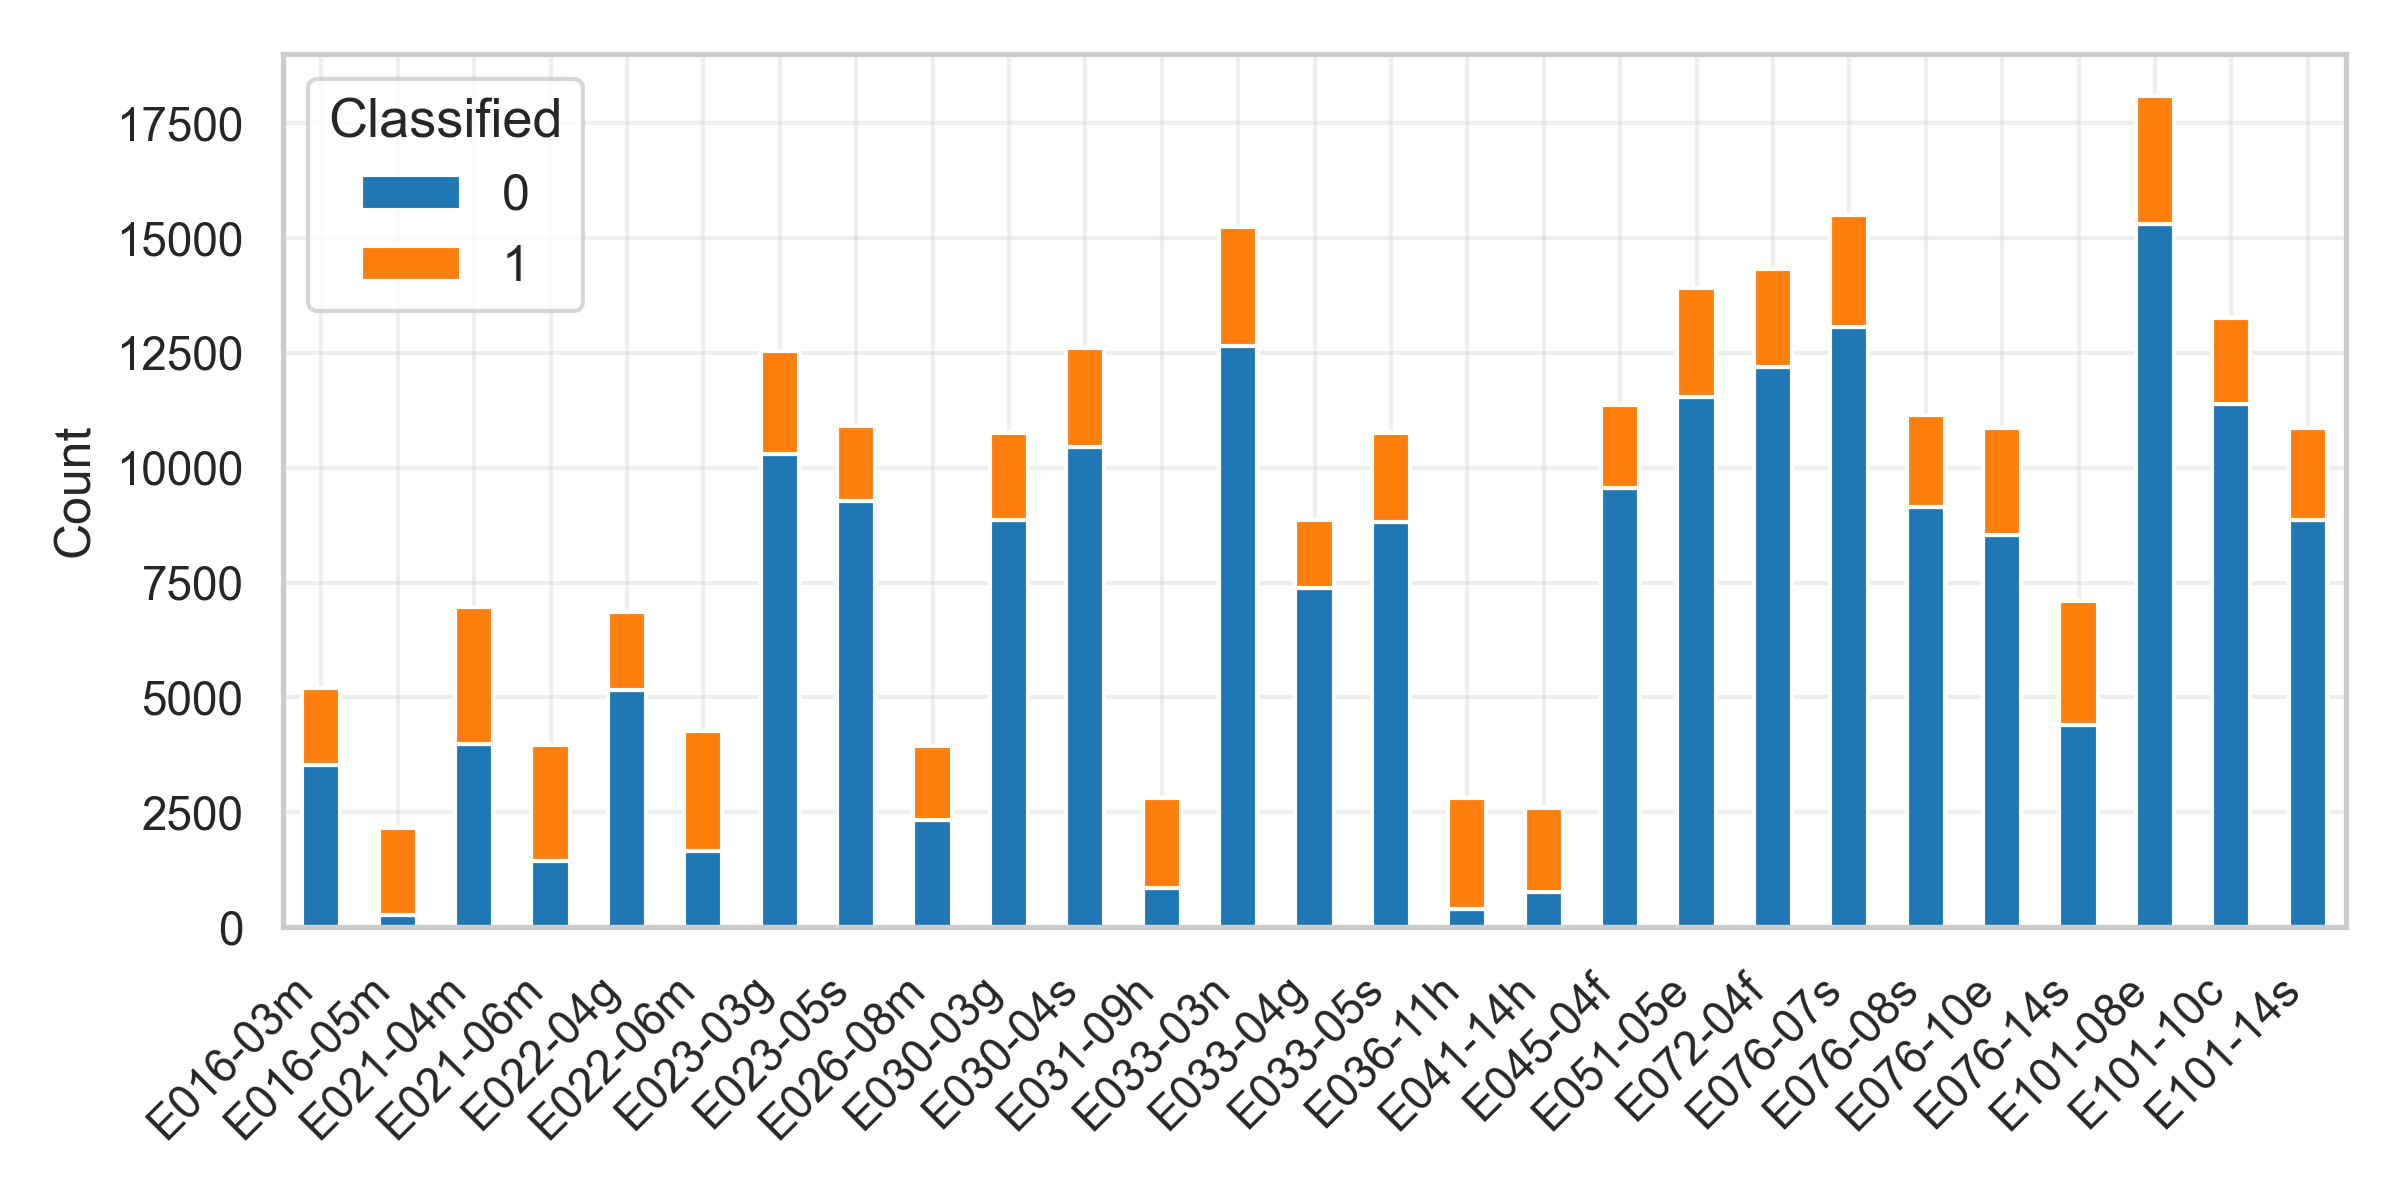
\includegraphics[width=\linewidth]{pictures/dataset_structure/distribution_plot_RandomData_5_40_40_10.png}
		\caption{RD-5-40-40-10.}
	\end{subfigure}%
	\begin{subfigure}[t]{.5\textwidth}
		\centering
		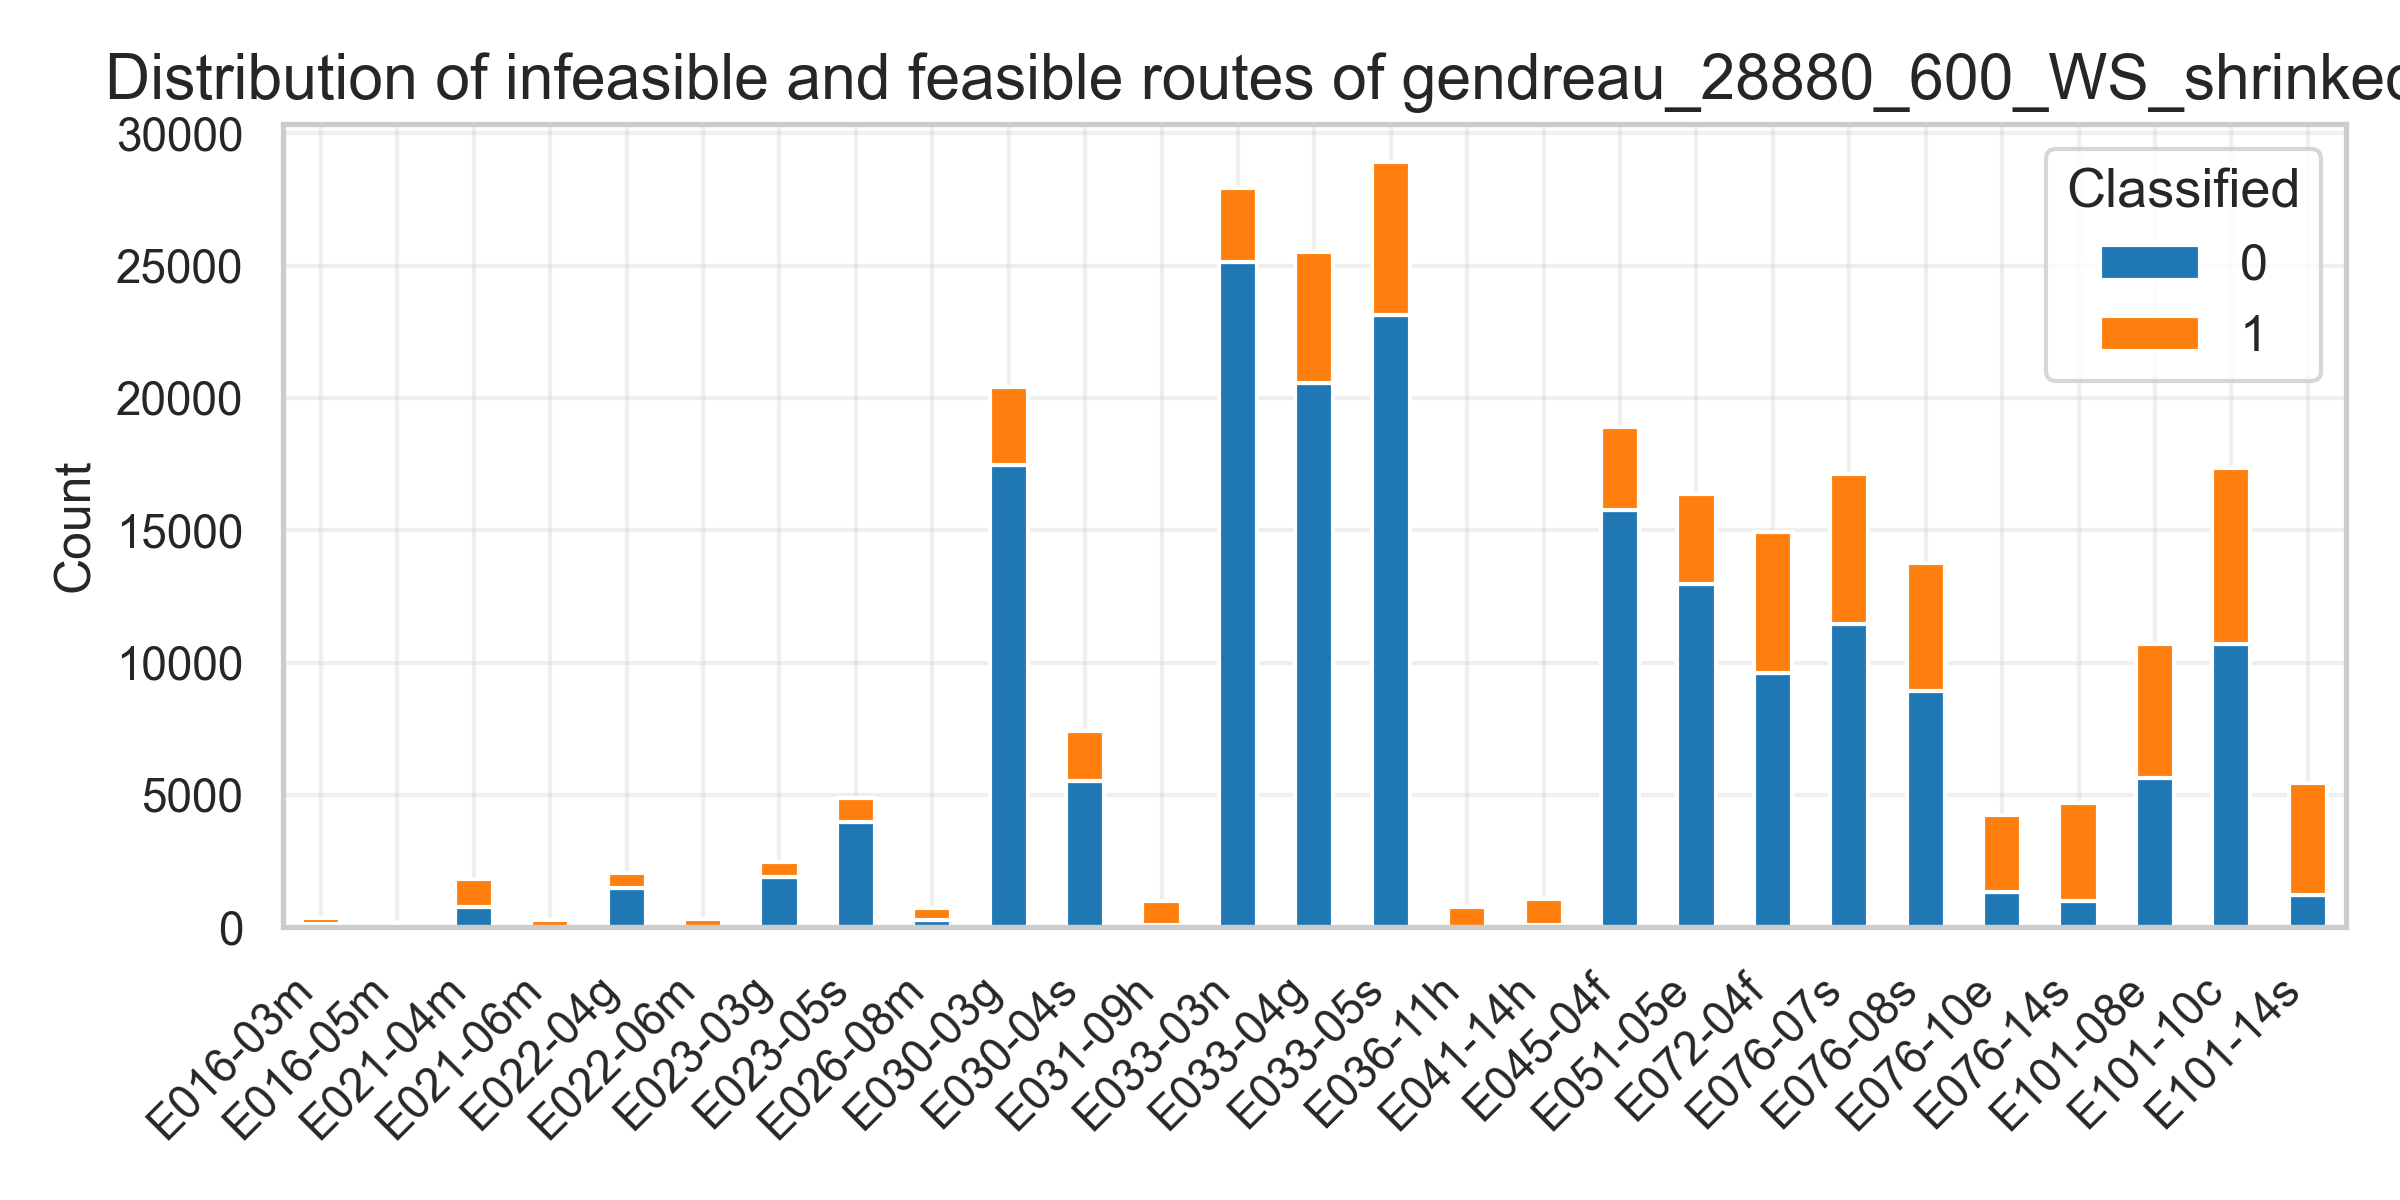
\includegraphics[width=\linewidth]{pictures/dataset_structure/distribution_plot_gendreau_28880_600_WS_shrinked094.png}
		\caption{Complete-Shrunken-WS.}
	\end{subfigure}
	\caption[Distribution of routes considered per instance for two exemplary datasets of random and save strategy.]
	{Distribution of routes considered per instance for two exemplary datasets of random and save strategy.}
	\label{fig:comparison_noroutes_perInstancce}
\end{figure}

\subsection{Feature Filter Results}
\label{sec:feature_filter_results}

The filter algorithm (Algorithm~\ref{alg:filter_algorithm}) was applied using minimum importance thresholds $\epsilon \in {0.1, 0.2, 0.3, 0.4}$
and barrier values $\mathcal{B} \in {0.5, 0.75}$. In addition, pearson correlation thresholds $\Phi \in {0.8, 0.85, 0.9}$ were considered
across all 27 datasets $\mathcal{D}$ introduced in the previous subsection. Figure~\ref{fig:feature_filter_parameters} in the appendix
illustrates how the drop sets are constructed by varying $\epsilon$ and $\mathcal{B}$. Importance thresholds below 20\% were also tested, but
did not affect the final subsets. The specific features removed under each configuration are listed in Table~\ref{tab:feature_dropsets},
while Table~\ref{tab:drop_set_presentation_shortened} summarizes the drop set names and the number of features excluded. The drop set
names have the following structure: DS-$100\mathcal{B}$-$10\epsilon$. For comparison purposes an additional empty drop set (DS-0-0) was included.

\begin{table}[ht]
	\centering
	\small
	\begin{tabular}{l c c c c c c c}
		\toprule
		Drop Set Name         & DS-0-0 & DS-50-2 & DS-50-3 & DS-50-4 & DS-75-2 & DS-75-3 & DS-75-4 \\
		\midrule
		Barrier $\mathcal{B}$ & -      & 0.5     & 0.5     & 0.5     & 0.75    & 0.75    & 0.75    \\
		Threshold $\epsilon$  & -      & 0.2     & 0.3     & 0.4     & 0.2     & 0.3     & 0.4     \\
		Number Features       & 0      & 10      & 18      & 38      & 7       & 18      & 32      \\
		\bottomrule
	\end{tabular}
	\caption{Considered drop sets for the feature selection.}
	\label{tab:drop_set_presentation_shortened}
\end{table}
For each drop set, every dataset was trained with each model type and then used to predict the
true labels of all other datasets in order to identify the best-performing drop set. The hyperparameters used for
each model are provided in Table~\ref{tab:hyperparams_feature_selection} in the appendix. For the subsequent analysis,
results obtained from predicting between datasets of the save strategy were excluded, since these datasets are nested
subsets of one another (see Table~\ref{tab:saved_instances_gendreau}). Figure~\ref{fig:mcc_filter_results} presents boxplots of
the \gls{MCC} for all drop sets and the three model types introduced in Section~\ref{sec:modelselection}.

\begin{figure}[ht]
	\centering
	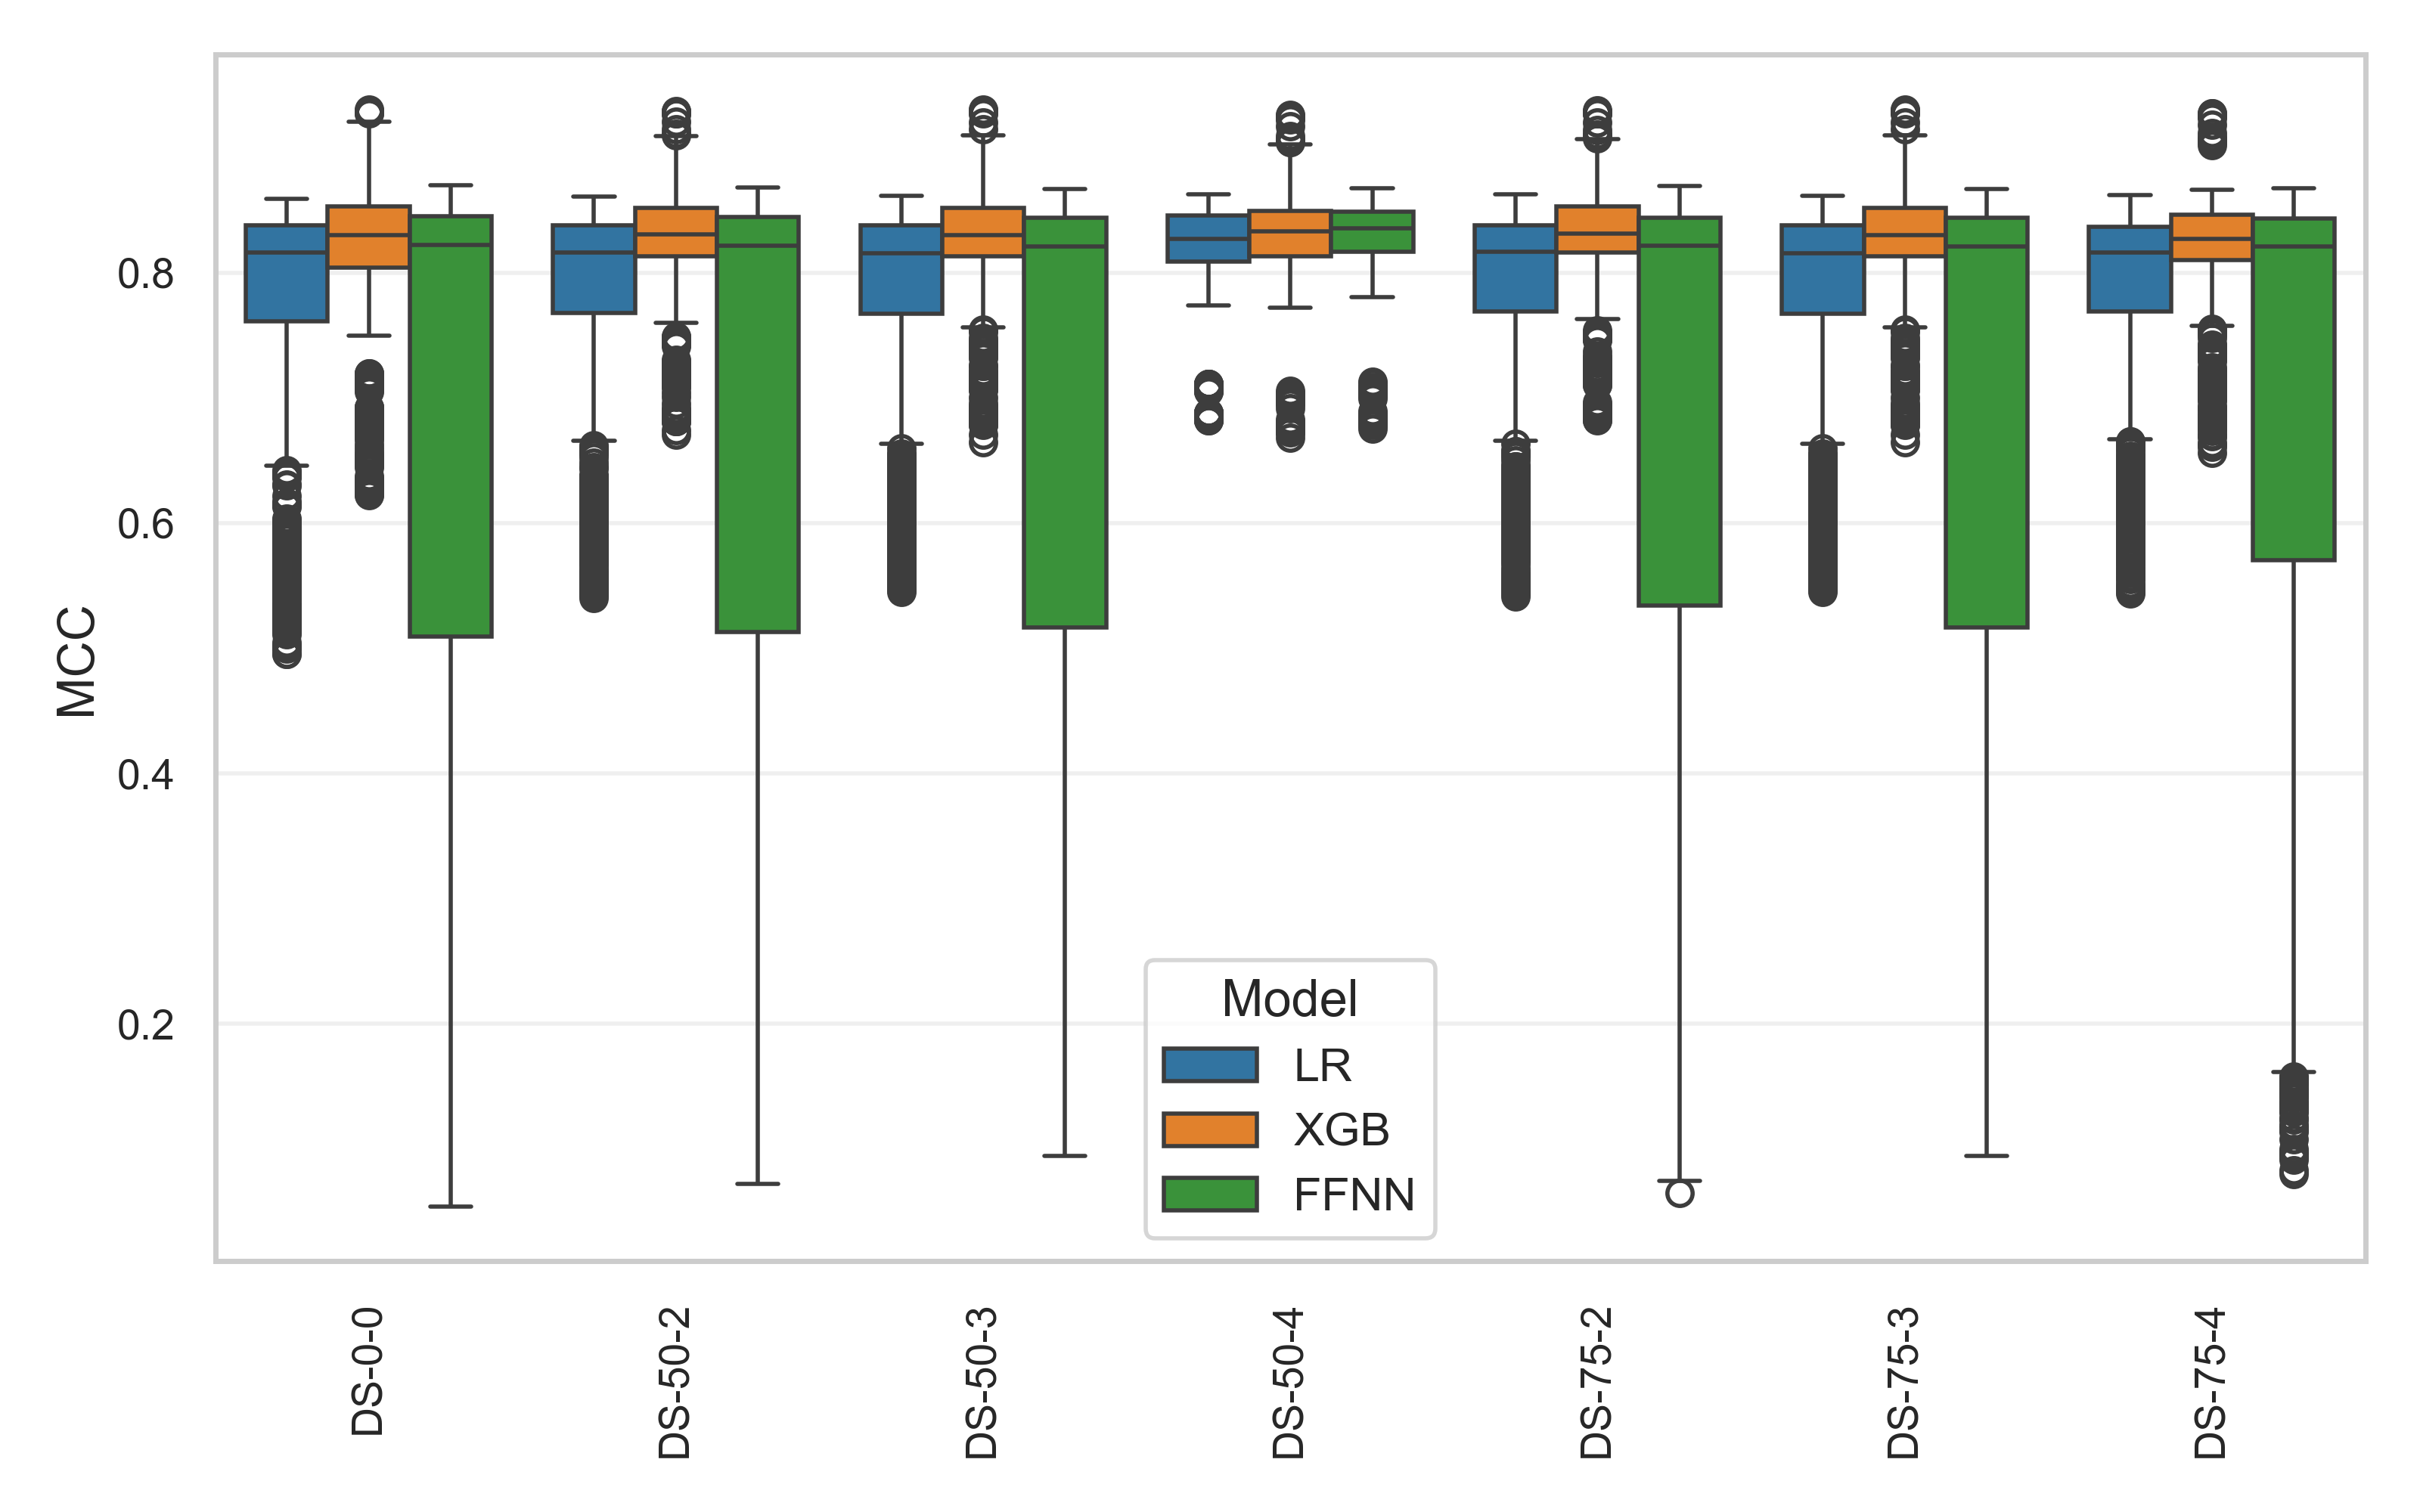
\includegraphics[width = .85\textwidth]{pictures/feature_filter/all_data_exceptSubsets_box_plot.png}
	\caption{Box plots of MCC performance of different feature drop sets.}
	\label{fig:mcc_filter_results}
\end{figure}
Two main observations can be drawn from the boxplot. First, the \gls{FFNN} model exhibits the widest variation in performance, whereas the XGB model
shows the smallest. Second, drop set DS-50-4 achieves the most consistent results across datasets. For both LR and FFNN, the performance
spread is larger than for XGB due to the need to scale the data before making predictions and to incorporate all features in the prediction.
Since scaling depends on the statistics of
the training dataset (e.g., mean and standard deviation), differences in dataset structure\footnote{Compare Table~\ref{tab:saved_instances_gendreau} and Table~\ref{tab:created_instances_xyz_gendreau} for the created datasets.}
can lead to mismatched feature ranges in the prediction datasets, thereby reducing performance. The \gls{FFNN} model is particularly sensitive
to such mismatches, as the hidden layers amplify these effects more strongly than in LR. Drop set DS-50-4, which removes 38 of
the 48 initial features, mitigates this issue by reducing complexity and minimizing the risk of mis-scaling, while still
achieving predictive performance comparable to other drop sets, as seen in the boxplot comparison. The full set of results across
all performance metrics is presented in Table~\ref{tab:featurePerformance_Alldata}.

\begin{table}[ht]
	\centering
	\small
	\begin{tabular}{lrrrrrrr}
		\toprule
		Drop Set & DS-0-0 & DS-50-2 & DS-50-3 & DS-50-4       & DS-75-2 & DS-75-3 & DS-75-4 \\
		\midrule
		MCC      & 0.75   & 0.76    & 0.76    & \textbf{0.82} & 0.76    & 0.76    & 0.76    \\
		F1-Score & 0.81   & 0.82    & 0.82    & \textbf{0.88} & 0.82    & 0.82    & 0.82    \\
		Accuracy & 0.89   & 0.89    & 0.89    & \textbf{0.93} & 0.89    & 0.89    & 0.89    \\
		AUROC    & 0.96   & 0.96    & 0.96    & \textbf{0.98} & 0.95    & 0.96    & 0.96    \\
		\bottomrule
	\end{tabular}
	\caption[Mean performance metrics of different drop sets.]
	{Mean performance metrics of different drop sets excluding the prediction across save strategy datasets.
		Bold font shows the best results for each performance score.}
	\label{tab:featurePerformance_Alldata}
\end{table}

The final features considered for predicting the loading feasibility are the following:
\begin{table}[!ht]
	\centering
	\def\arraystretch{1.5}
	\begin{tabular}{l l l l }
		\sbt Rel Volume      & \sbt Fragile Sequence    & \sbt width-W-mean & \sbt height-H-std    \\
		\sbt  length-L-std   & \sbt Weight Distribution & \sbt width-W-std  & \sbt height-area-min \\
		\sbt  area-AREA-mean & \sbt area-AREA-max       &                   &                      \\
	\end{tabular}
\end{table}

Additional feature filter results are provided in Section~\ref{app:sec:further_feature_filter} of the appendix.
These confirm that drop set DS-50-4 achieves the best overall performance, while models requiring feature scaling generally perform worse
across multiple datasets. The following section addresses the selection of datasets to be used as classifiers in the final algorithm.

\subsection{Selection of dataset}
\label{sec:dataset_selection}

The feature filter performance analysis described in the previous section can be used to identify the best-performing datasets
from each retrieval strategy, when the results for drop set DS-50-4 are solely investigated. Figure~\ref{fig:dataset_performance_group_subgroup}
shows the \gls{MCC} performance as a function of the chosen base dataset (Group) and the subgroup of predicted datasets, which are either
random or save-strategy datasets. Here, BC stands for the save-strategy with the B\&C algorithm.
As noted earlier, for save-strategy datasets only the performance on the base dataset is considered,
since these datasets are subsets of one another.
\begin{figure}[ht]
	\centering
	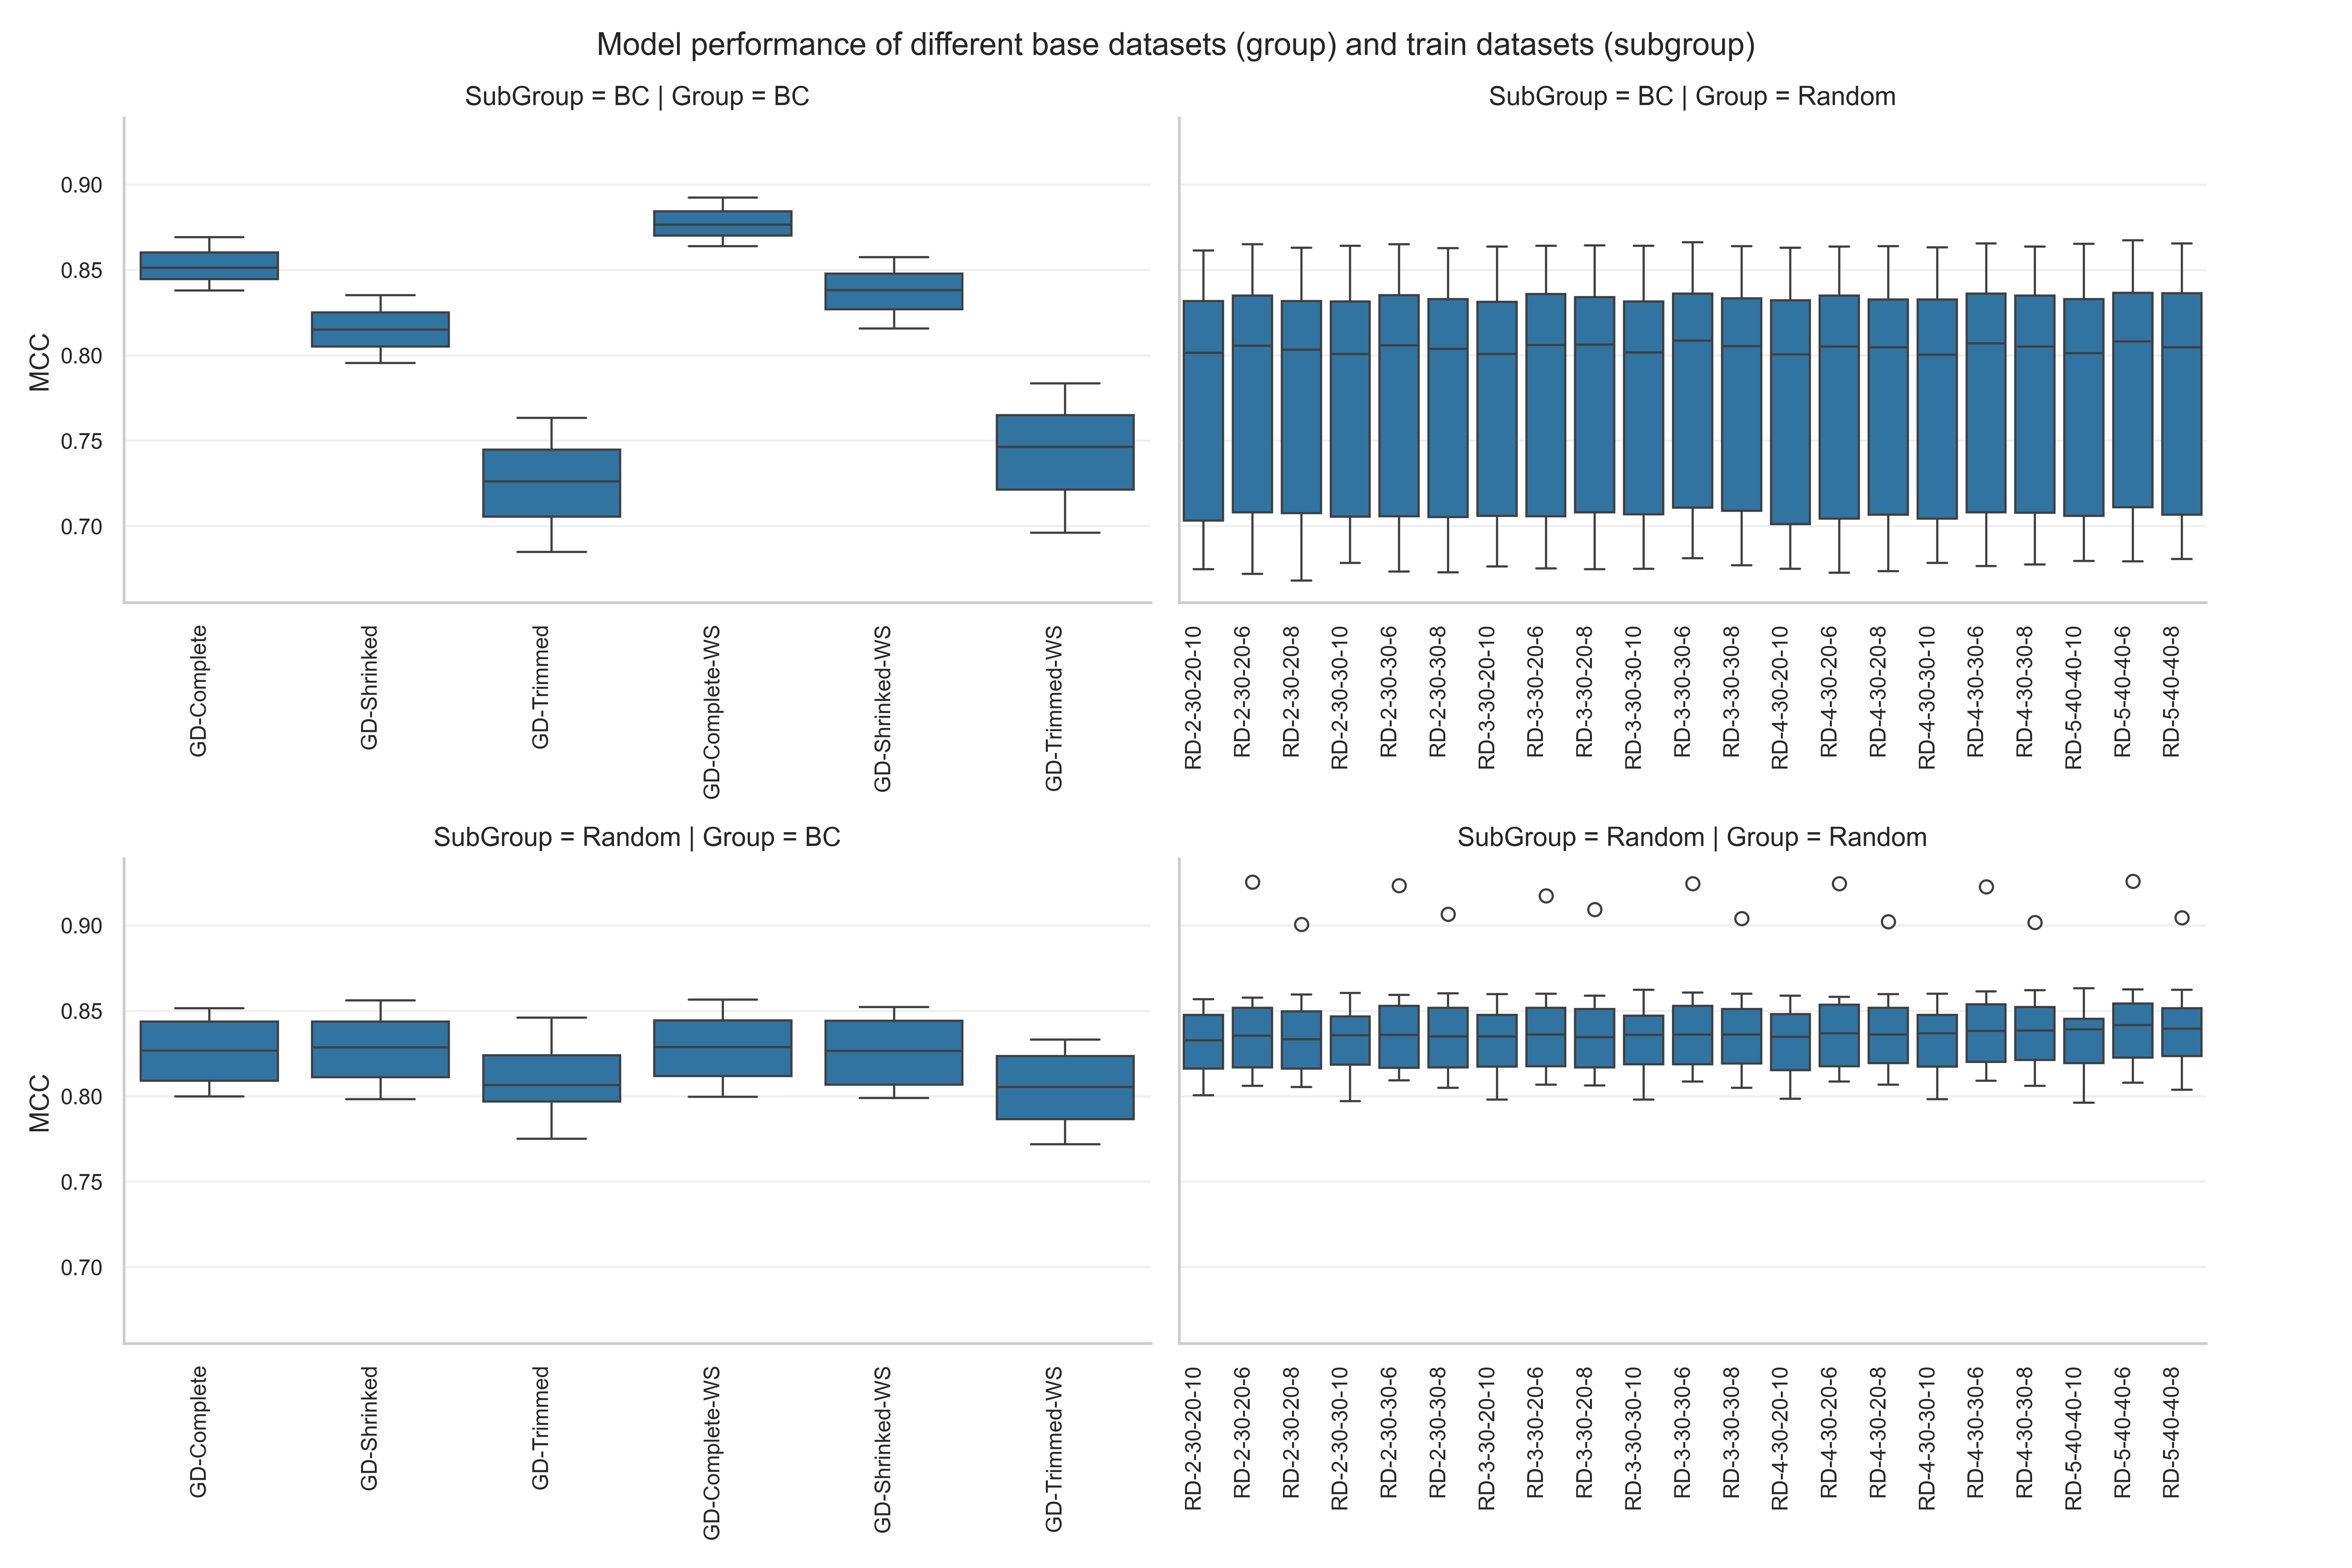
\includegraphics[width =\textwidth]{pictures/feature_filter/group_subgroup_results.png}
	\caption{Box plots of MCC performance of different feature drop sets.}
	\label{fig:dataset_performance_group_subgroup}
\end{figure}

In the first subplot, where Group = SubGroup = BC, only the performance on the base training dataset is
displayed for each respective model type (\gls{LR}, XGB, and \gls{FFNN}). This subset is the only one showing significant
performance differences, with the Complete datasets outperforming the others. When the subgroup consists of random datasets,
the performance of the Shrunken and Complete datasets is similar. The Trimmed datasets, however, can be excluded from consideration,
as their predictive capability is restricted by the lack of feasible small tours (only infeasible two-customer routes are included).
For the random dataset subgroup, the results are more difficult to interpret, as the median performance remains nearly constant
across datasets. Still, when both group and subgroup are random datasets, a slight improvement in median performance can
be observed for smaller values of $\delta$ within the same ($\alpha$, $\beta$, $\gamma$) parameter group. To avoid arbitrary dataset
selection, an additional validation dataset was constructed by saving the routes found during the base \gls{ILS} algorithm,
with feasibility checks carried out exclusively by the \gls{CP} solver. Each instance from \gendreauDataSetText was run
five times with different seeds and an extended time limit of 15 minutes to generate a large set of candidate routes.
The parameters used for this run are provided in Table~\ref{tab:parameters_final_noclassifier} and
the validation dataset characteristics are displayed in the Table~\ref{tab:validation_dataset_gendreau}.
\begin{table}[!ht]
	\centering
	\small
	\begin{tabular}{l c c c c c }
		\toprule
		Name          & Routes & Route Len = 2 & Balance   & Rel. Vol & Rel. Mass \\
		\midrule
		Validation DS & 427048 & 8605          & 47.0/53.0 & 0.61     & 0.60      \\
		\bottomrule
	\end{tabular}
	\caption{Characteristics of validation dataset constructed from \gendreauDataSetText with NoClassifier iterated local search algorithm.}
	\label{tab:validation_dataset_gendreau}
\end{table}

The datasets contains many rows with a balanced profile of feasible and infeasible labels. In comparison to both
random and save-strategy datasets the number of routes with two customers is very low, as the \gls{ILS} algorithm
works with dense routes to improve the solution quality. The \gls{MCC} score for every model and train dataset
from random and save strategy is shown in the following Figure~\ref{fig:validation_performance_line_plot}.

\begin{figure}[ht]
	\centering
	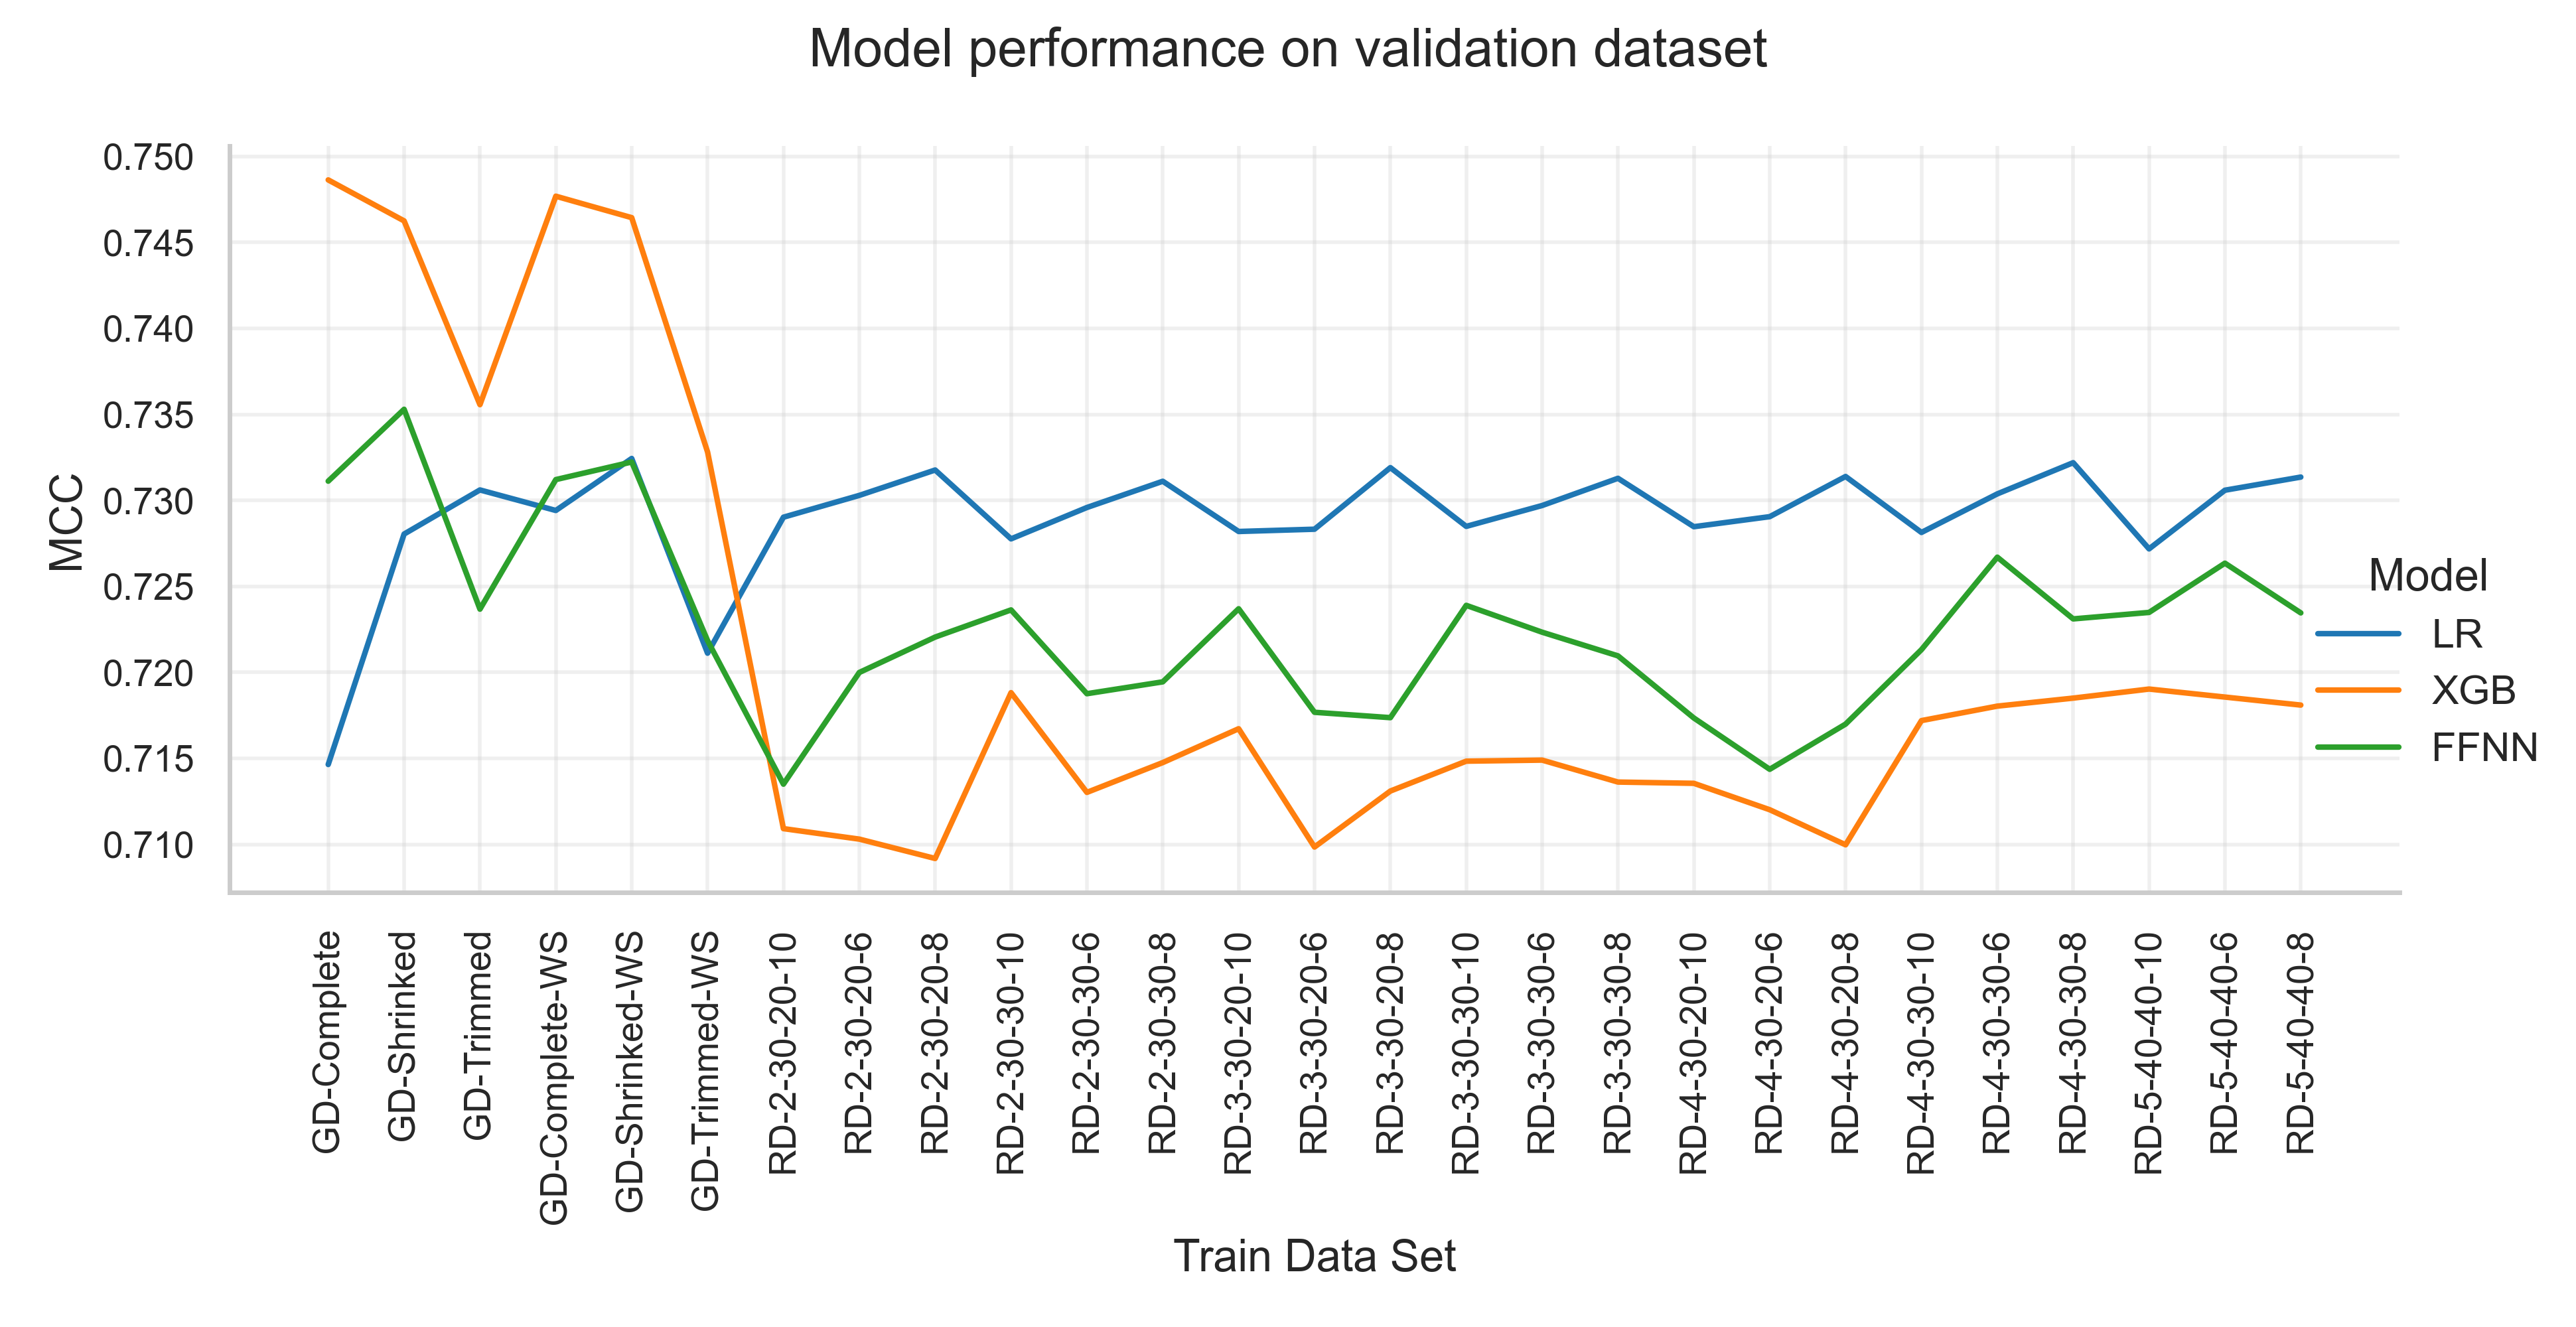
\includegraphics[width =\textwidth]{pictures/feature_filter/validation_line_plot.png}
	\caption{Obtained MCC from validation dataset based on different train datasets and model types.}
	\label{fig:validation_performance_line_plot}
\end{figure}

With the exception of the trimmed datasets, the save-strategy datasets generally achieve better predictive performance.
However, the \gls{MCC} scores, independent of the training dataset, are significantly lower than those shown in
Figure~\ref{fig:dataset_performance_group_subgroup}. While the \gls{LR} model yields consistent values across dataset groups,
the performance of XGB and FFNN decreases when trained on random-strategy datasets, reversing the ranking of the best-performing
models from one group to the other. This motivates a more detailed comparison of solution quality with respect to dataset type and
its causal relationship with model choice. The complete results for all performance metrics are reported in Table~\ref{tab:featurePerformance_validationDataset},
with the best values highlighted in bold. The following four datasets are used in the further analysis.
\begin{table}[ht]
	\centering
	\small
	\setlength{\tabcolsep}{0.75em}
	\def\arraystretch{1.25}
	\begin{tabular}{lll}
		\toprule
		Save Strategy   & GD-Shrunken  & GD-Shrunken-WS \\\midrule
		Random Strategy & RD-4-30-30-6 & RD-4-30-30-8   \\
		\bottomrule
	\end{tabular}
	\caption{Chosen datasets for training final classifier.}
	\label{tab:chosen_datasets}
\end{table}
The choice of the four datasets is based on their superior performance among the evaluation metrics,
but also on the need to compare random versus save-strategy datasets and to examine whether adjusting the threshold $\delta$ or adding
more routes to the training dataset yields better results. With both the features and dataset determined, a comparative analysis of the
datasets can be conducted. Figure~\ref{fig:feature_space} compares the feature space of the two datasets GD-Shrunken and RD-4-30-30-6,
illustrating the distribution of each feature. Interestingly, for the 10 selected features, the feature spaces are nearly identical,
with the largest differences arising from the large number of two-customer routes in the save-strategy dataset.
Figure~\ref{fig:distribution_cp_label} illustrates how the feature space can be divided into
feasible and infeasible labeled distributions, for the same dataset. For both plots, it is evident that, except for the feature relative volume,
no clear boundary exists between feasible and infeasible labels. Only the combination of multiple features allows a clear
separation of the labels.

\section{Parameter Study}
\label{sec:parameter_study}

The parameter study is divided in four subsections following the variants of the \gls{ILS} algorithm
presented in Section~\ref{sec:FeasibilityCheck}. This study follows a hierarchical procedure
tuning the parameters, introduced for each variant, sequentially. The following subset of 13
instances from \gendreauDataSetText is used:


\begin{table}[ht]
	\centering
	\setlength{\tabcolsep}{0.75em}
	\def\arraystretch{1.5}
	\begin{tabular}{lllllll}
		E016-03m & E022-04g & E023-03g & E023-05s & E030-03g & E033-04g & E033-05s \\
		E051-05e & E072-04f & E076-07s & E076-14s & E101-10c & E101-14s &          \\
	\end{tabular}
\end{table}

The division followed this approach. First all instances were omitted, which found
the optimal solution in a short time (see \cite{tamke_branch-and-cut_2024}\footcite[cf.][p. 26]{tamke_branch-and-cut_2024}).
Second, similar instances of size and complexity were reduced to only one.
Every instance is run three times with different seeds and a timelimit of 10 min. It will be investigated
how different parameter combinations influence the \gls{RPD}, the iteration number, the rejection rate and
the average improvement after finding the constructive solution. The \gls{RPD} is defined between the
total costs of the best solution $C^*$ and another solution with costs $C$.
\begin{align}
	RPD = \frac{C - C^*}{C^*} \cdot 100\%
\end{align}
The rejection rate is the proportion of iterations rejected as infeasible in the \gls{CP} check, which needs
to be applied after the SpeedUp and Hybrid  variant. These variants allow the acceptance of
new solutions only based on the classification and need to be checked for false positive predicted routes afterwards.

\subsection{NoClassifier Variant}
\label{subsec_parameterStuy_noclassifier}
In this variant, all base \gls{ILS} parameters are tested, providing the foundation for subsequent variants,
with the limitation that loading is checked only using the exact \gls{CP} solver. The following levels of
different parameters were tested in a full grid parameter study.
\begin{table}[ht]
	\centering
	\small
	\setlength{\tabcolsep}{2em}
	\def\arraystretch{1.1}
	\begin{tabular}{@{}L{4cm}P{8cm}@{}}
		\toprule
		Parametertype      & Levels                                                         \\
		\midrule
		AttemptsLimit $a$  & 3, 5, 8, 12                                                    \\
		RandomMoves R      & 2, 4, 8, 12                                                    \\
		Perturbation       & R-Swaps, R-Insertions, Both-Insertions-First, Both-Swaps-First \\
		Neighborhood order & IntraFirst, InterFirst                                         \\
		\bottomrule
	\end{tabular}
	\caption{Parameter levels for NoClassifier variant.}
	\label{tab:parameters_noclassifier}
\end{table}
The core result is, that the \gls{ILS} without speedups relies heavily on the number of iterations to find high-quality solutions.
For some instances, the average number of ILS iterations is very low, as shown in Figure~\ref{fig:average_iterations_noclassifier}.
To account for this, the instances were divided into two groups depending on whether the average number of iterations was below 25
(visualized with different bar colors and the horizontal red line). The heatmap of the parameters RandomMoves and LimitNoImpr
(Figure~\ref{fig:heatmap_parameter_study}) indicates that the best solutions were either found, when very few perturbations were
executed or when the search was frequently reset to the best solution found so far, thereby limiting the number of intensification
phases starting from a strongly perturbed solution.
\begin{figure}[ht]
	\centering
	\begin{minipage}[t]{0.49\textwidth}
		\centering
		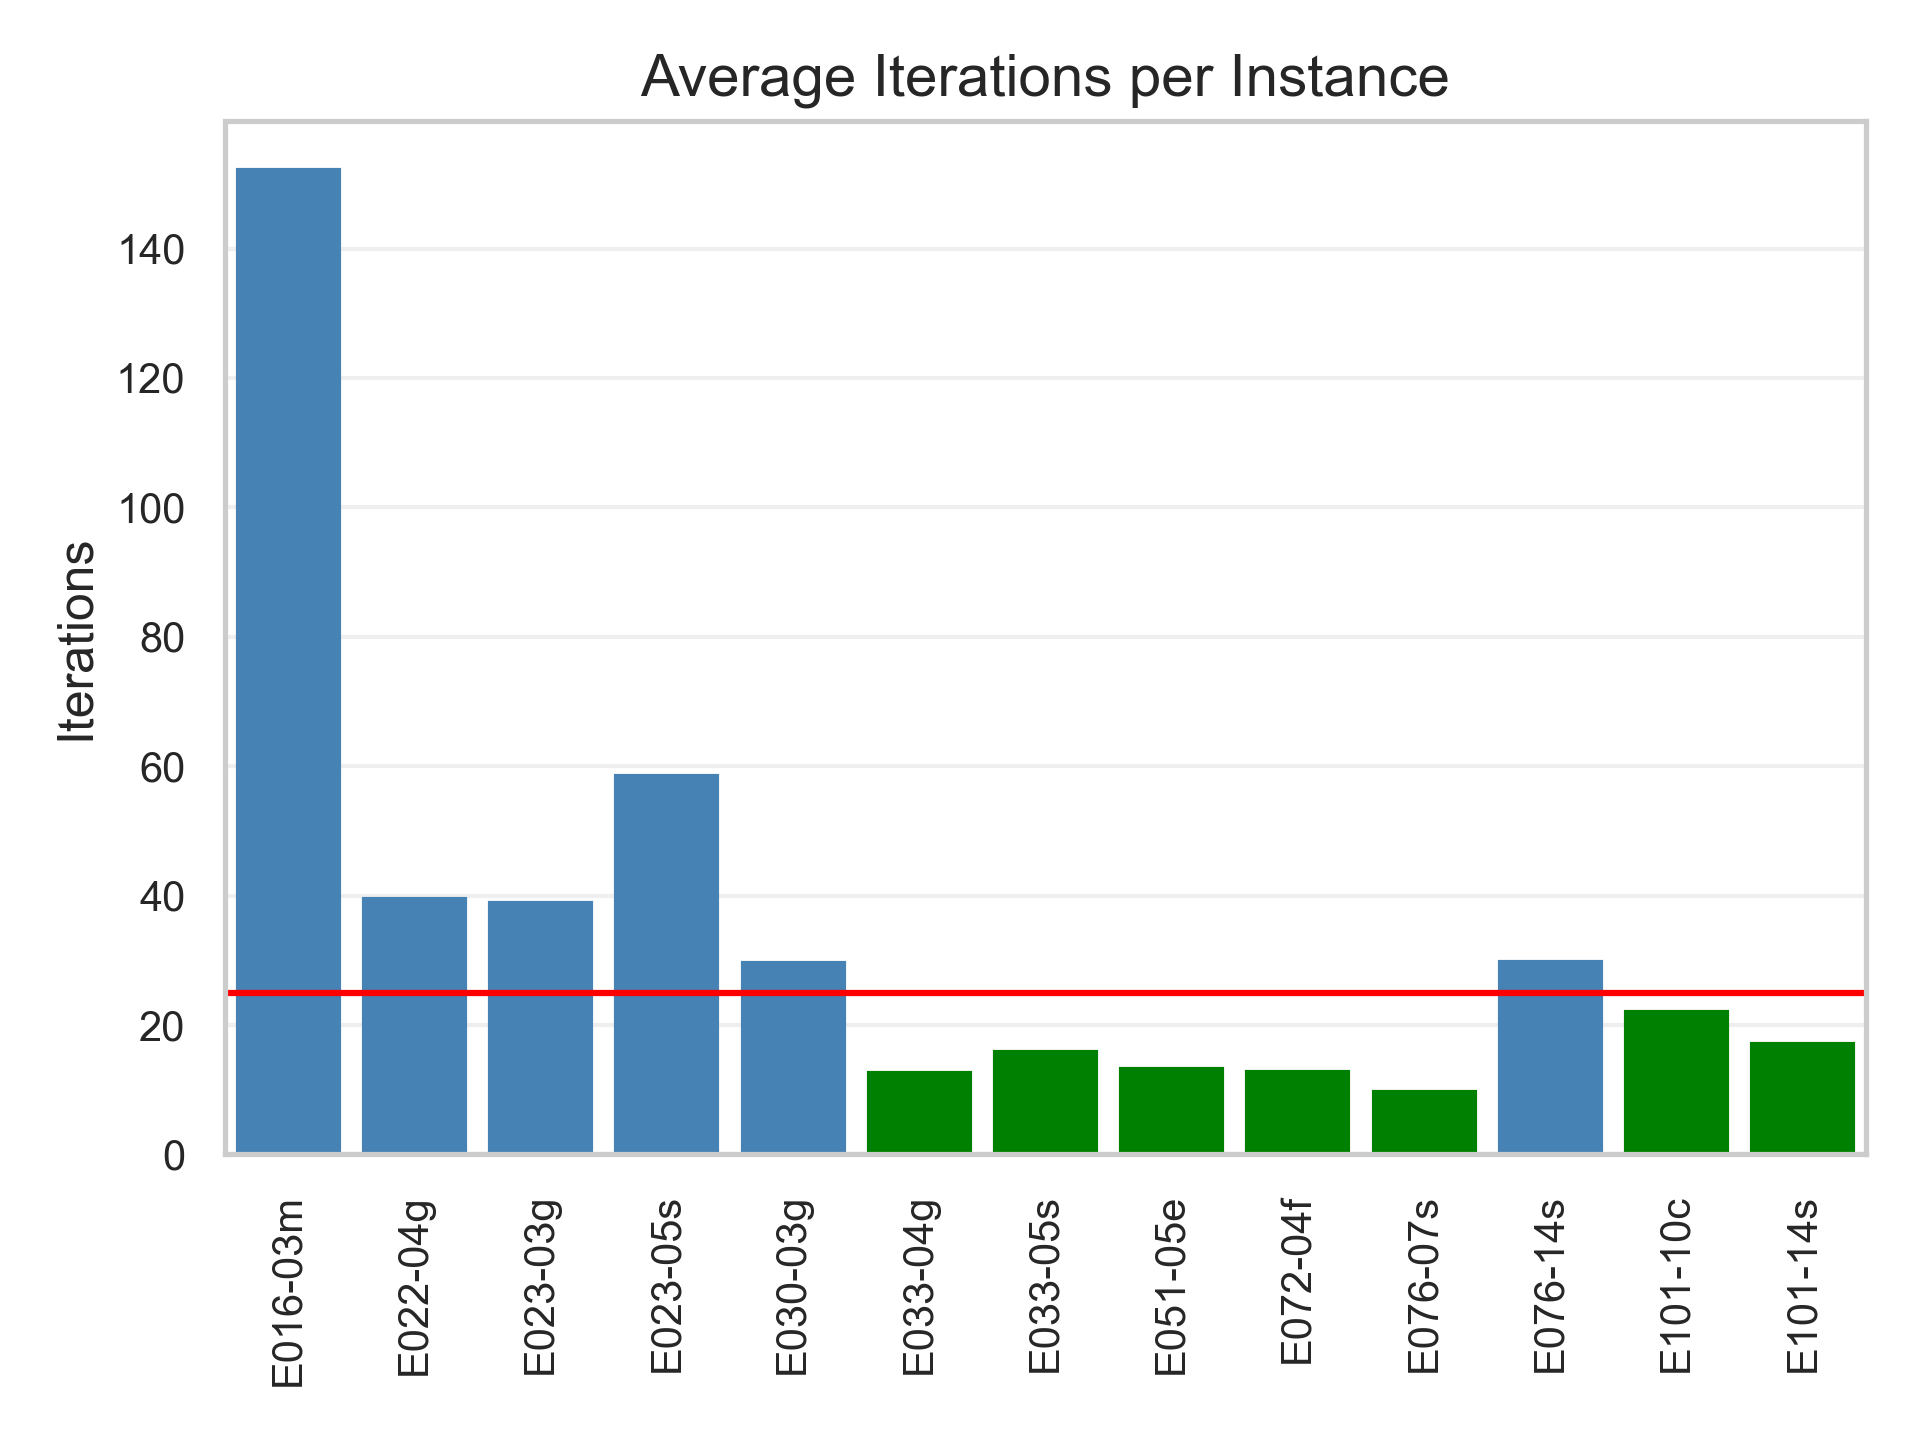
\includegraphics[width=\linewidth]{pictures/iterations_per_instance.png}
		\captionof{figure}{\small Average iterations for each \gendreauDataSetText instance.}
		\label{fig:average_iterations_noclassifier}
	\end{minipage}\hfill
	\begin{minipage}[t]{0.49\textwidth}
		\centering
		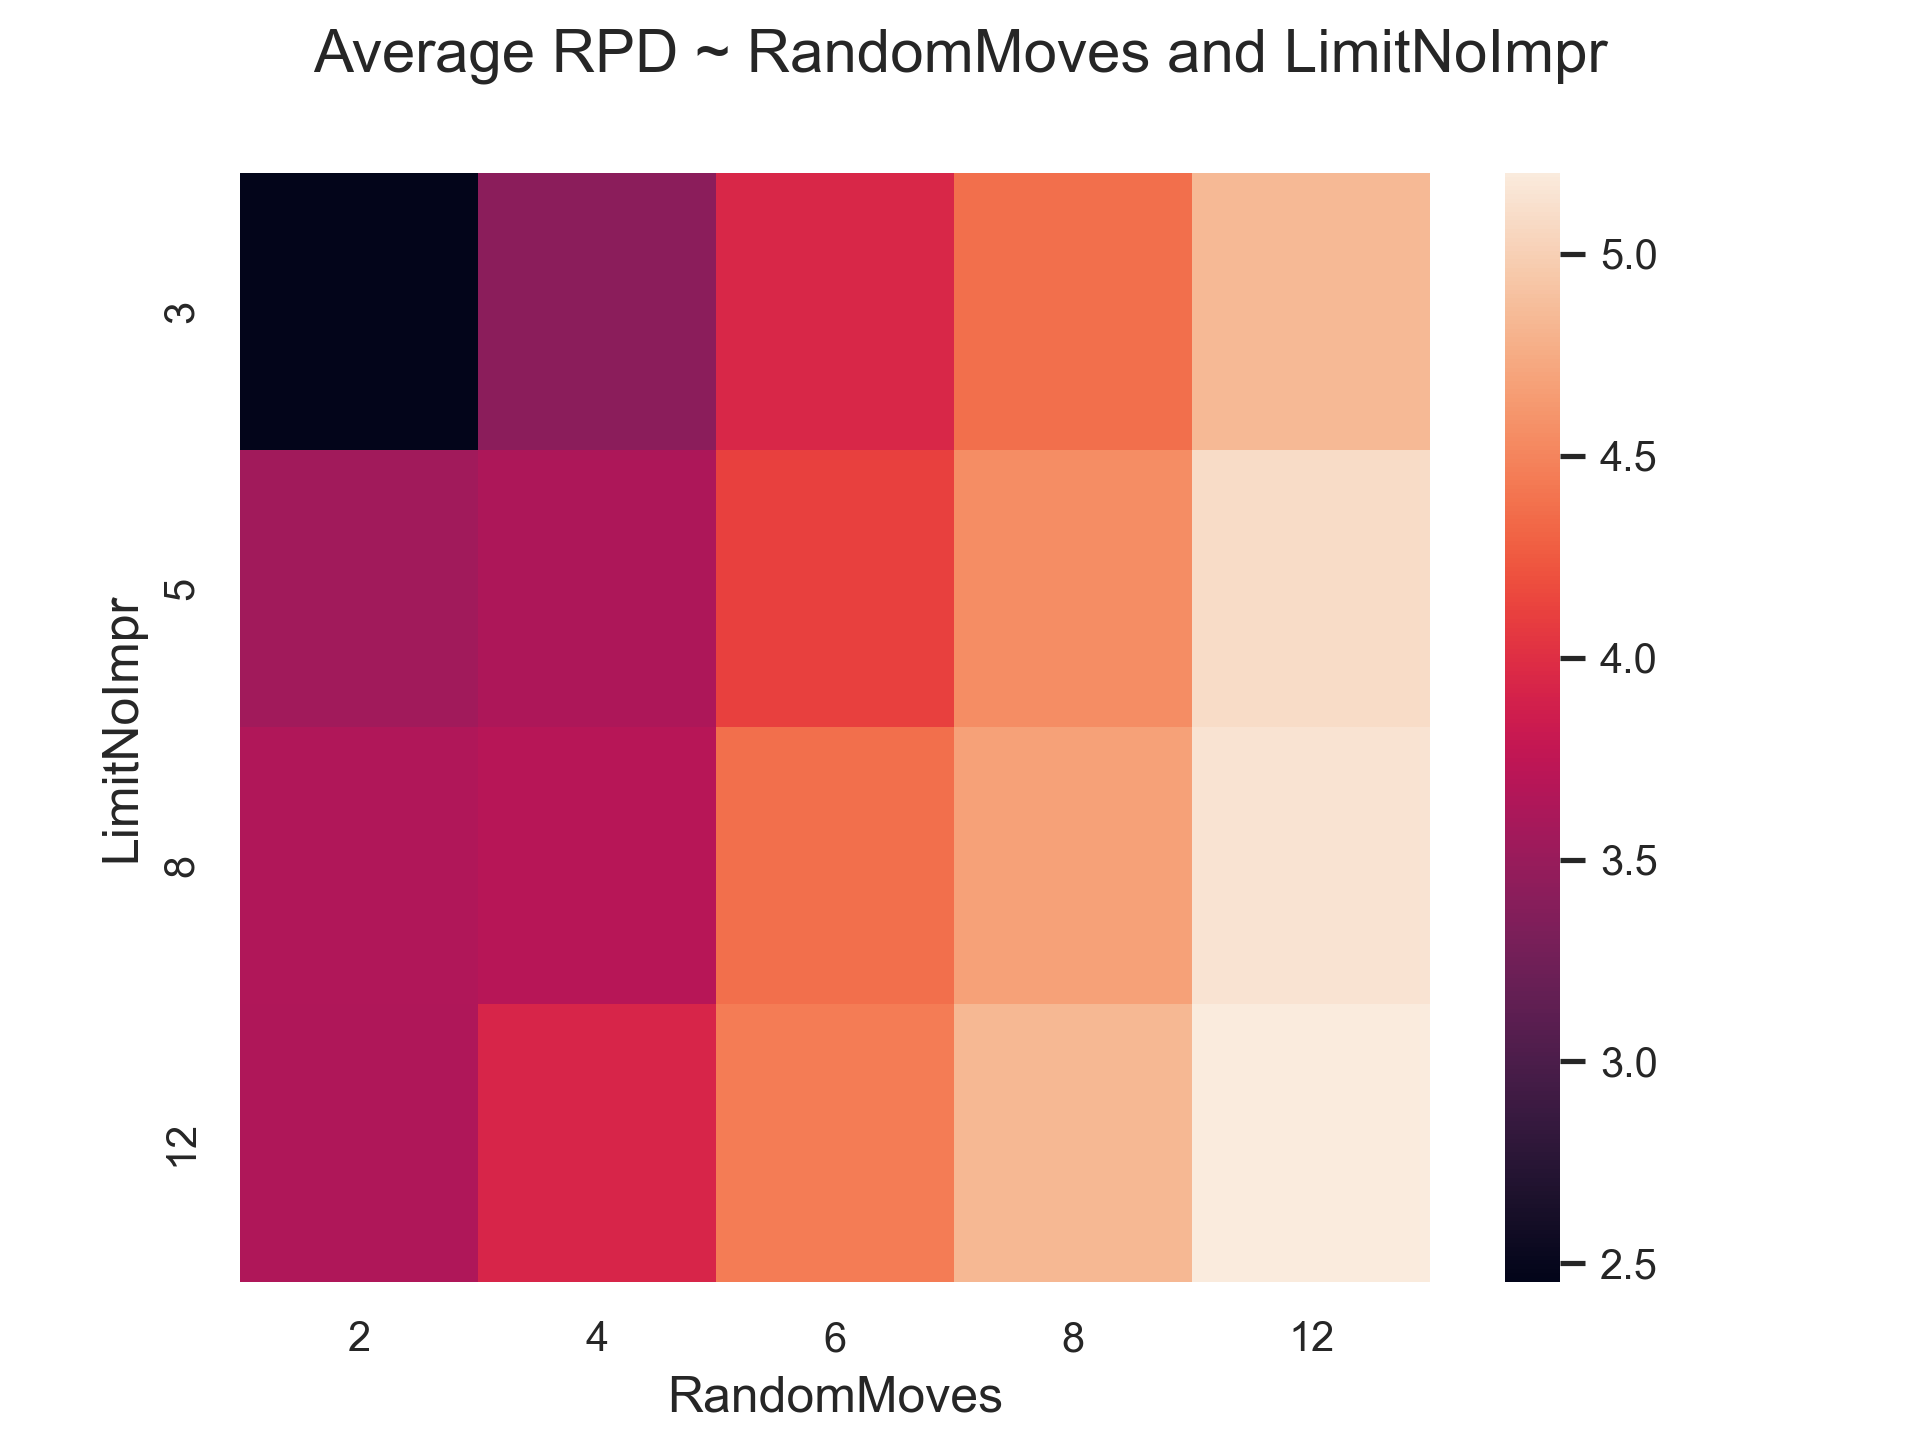
\includegraphics[width=\linewidth]{pictures/heatmap_randomMoves_limitNoImpr.png}
		\captionof{figure}{\small Dependency between RPD and RandomMoves and LimitNoImpr}
		\label{fig:heatmap_parameter_study}
	\end{minipage}
\end{figure}

The complete results are presented as boxplots for each parameter and performance metric in Figure~\ref{app:subsec:parameterstudy_noclassifier},
with corresponding numerical values in Table~\ref{tab:numerical_results_paramStudy_NOclassifiers}. Overall, the number of
iterations emerges as the dominant factor influencing performance. Dividing the instances into two groups (below and above 25 iterations)
reveals that several parameters behave quite differently across these groups.
Among all tested parameters, only the order of local-search neighborhoods significantly improves results in both groups, yielding a
1.78\% \gls{RPD} advantage when inter-neighborhoods are applied first. By contrast, other \gls{ILS} variants incorporate speedups,
enabling more iterations to be executed. In these cases, parameter effects are less about raw iteration count and more about
interaction patterns that extend beyond simply maximizing iterations. To keep the subsequent parameter study tractable,
a set of base parameters was defined to use in the upcoming analysis and as the configuration for the \textit{NoClassifier} variant.
This set represents a compromise between the results reported in Appendix~\ref{app:subsec:parameterstudy_noclassifier} for instances with
many versus few iterations.

\begin{table}[ht]
	\centering
	\small
	\begin{tabular}{@{}cccc@{}}
		\toprule
		AttemptsLimit & RandomMoves        R & Local Search order & Perturbation          \\
		\midrule
		3             & 4                    & InterLSFirst       & Both-Insertions-First \\
		\bottomrule
	\end{tabular}
	\caption{Chosen parameters for the NoClassifier iterated local search variant.}
	\label{tab:parameters_final_noclassifier}
\end{table}

\subsection{Classifier Variants}
\label{subsec_parameterStuy_speedup}
For the parameter study of the classifier variants, a single dataset (GD-Shrunken-WS) is used. This choice is motivated
by the fact that classifier behavior is independent of the dataset, while performance differences are instead revealed in
the comparison between the NoClassifier baseline and the classifier-based variants. The study is summarized in
Table~\ref{tab:parameters_summary_classifier}, with detailed results for all parameter levels presented in the Appendix,
where hyperlinks are provided for quick reference.
In the analysis, several aspects are examined. For all classifier variants, it is investigated whether the Filter strategy
within the constructive heuristic offers an advantage. For the SpeedUp and Hybrid variants, the study additionally
considers whether allowing multiple iterations without a \gls{CP} check can improve performance. Within the Hybrid variant,
further attention is given to identifying the most suitable component of the algorithm, intra \gls{LS}, inter \gls{LS}, or
perturbation, for the use of the \gls{CP} solver.
\begin{table}[ht]
	\centering
	\def\arraystretch{1.2}
	\begin{tabular}{@{}l l c c@{}}
		\toprule
		Variant                  & Parameter                & Levels                                                & Appendix                                                 \\
		\midrule
		\multirow{1}{*}{Filter}  & UseFilterStartSolution   & True, \textbf{False}                                  & \multirow{1}{*}{\ref{app:subsec:parameterstudy_Filter}}  \\\midrule
		\multirow{2}{*}{SpeedUp} & IterationsWithoutCPCheck & \textbf{1},3,5                                        & \multirow{2}{*}{\ref{app:subsec:parameterstudy_SpeedUp}} \\
		                         & UseFilterStartSolution   & True, \textbf{False}                                  &                                                          \\
		\midrule
		\multirow{3}{*}{Hybrid}  & IterationsWithoutCPCheck & \textbf{1},3,5                                        & \multirow{3}{*}{\ref{app:subsec:parameterstudy_Hybrid}}  \\
		                         & Hybrid Usage             & Perturbation, \textbf{Inter \gls{LS}}, Intra \gls{LS} &                                                          \\
		                         & UseFilterStartSolution   & True, \textbf{False}                                  &                                                          \\
		\bottomrule
	\end{tabular}
	\caption[Summary of parameter levels for classifier Variants.]{Summary of parameter levels for classifier variants and links to visualizations in appendix. Chosen parameter level is highlighted in bold font.}
	\label{tab:parameters_summary_classifier}
\end{table}

The numerical results and the median values for each parameter level are shown in Table~\ref{tab:numerical_results_paramStudy_classifiers}.
The following analysis is based on the median results, which are comparable with the boxplots.
In general, the use of the Filter variant in the constructive phase leads to worse \gls{RPD} results across all variant types,
with an average difference of 1.1\%. Despite this, the number of iterations increased by 16.8\% and 15.8\% for the Filter and Hybrid variants,
respectively. The SpeedUp variant showed the smallest increase in iterations (4.4\%), yet it achieved by far the highest median
number of iterations overall, followed by the Hybrid and then the Filter variant. The filter start solution wont be further used for any variant to
keep the results comparable. Increasing the interval of the \gls{CP} check consistently resulted in more iterations. For the Hybrid variant,
the increase from level 1 to level 5 was modest at 12.2\%, while for the SpeedUp variant it was substantial at 127.6\%. However, for both
variants, the rejection ratio nearly doubled across these levels, and the \gls{RPD} results deteriorated. This indicates that checking the solution
at every iteration yields the best overall performance. The parameter choice of which component to apply the \gls{CP} check to in the Hybrid variant also produced notable differences.
The best \gls{RPD} was achieved when the intra \gls{LS} was checked with the \gls{CP} solver, as this setting allowed at least three times more
iterations than the other alternatives. The rejection rate varied considerably: 57\% for InterCPSolver, 89\% for PerturbationCPSolver
and 69\% for IntraCPSolver. This suggests that the perturbation phase has the lowest impact on solution feasibility, while the inter-phase
has the highest. Conversely, the intra \gls{LS} phase is the least computationally intensive, as it allows the highest number of iterations
when paired with the \gls{CP} solver. Based on these findings, the InterCPSolver was selected as the setting for the final comparison.
The bold parameter levels in Table~\ref{tab:parameters_summary_classifier} highlight the chosen variant configuration.

\section{Comparison of ILS Variants}
\label{sec:comparison_ils_variants}

The solution quality for all four \gls{ILS} variants (see Fig.~\ref{fig:four_variants}) is compared by solving all 27 instances of the
\gendreauDataSetText dataset. The timelimit is set to 10 min and three runs are executed per instance with different seed values.
For every classifier based variant (Filter, SpeedUp, Hybrid) three different models (\gls{LR}, \gls{XGB},\gls{FFNN}) and four datasets
(see Table~\ref{tab:chosen_datasets}) are chosen, which results in a total of 37 different configurations. The four variants are compared
in Figure~\ref{fig:boxplots_final_comparison}.
\begin{figure}[!ht]
	\centering
	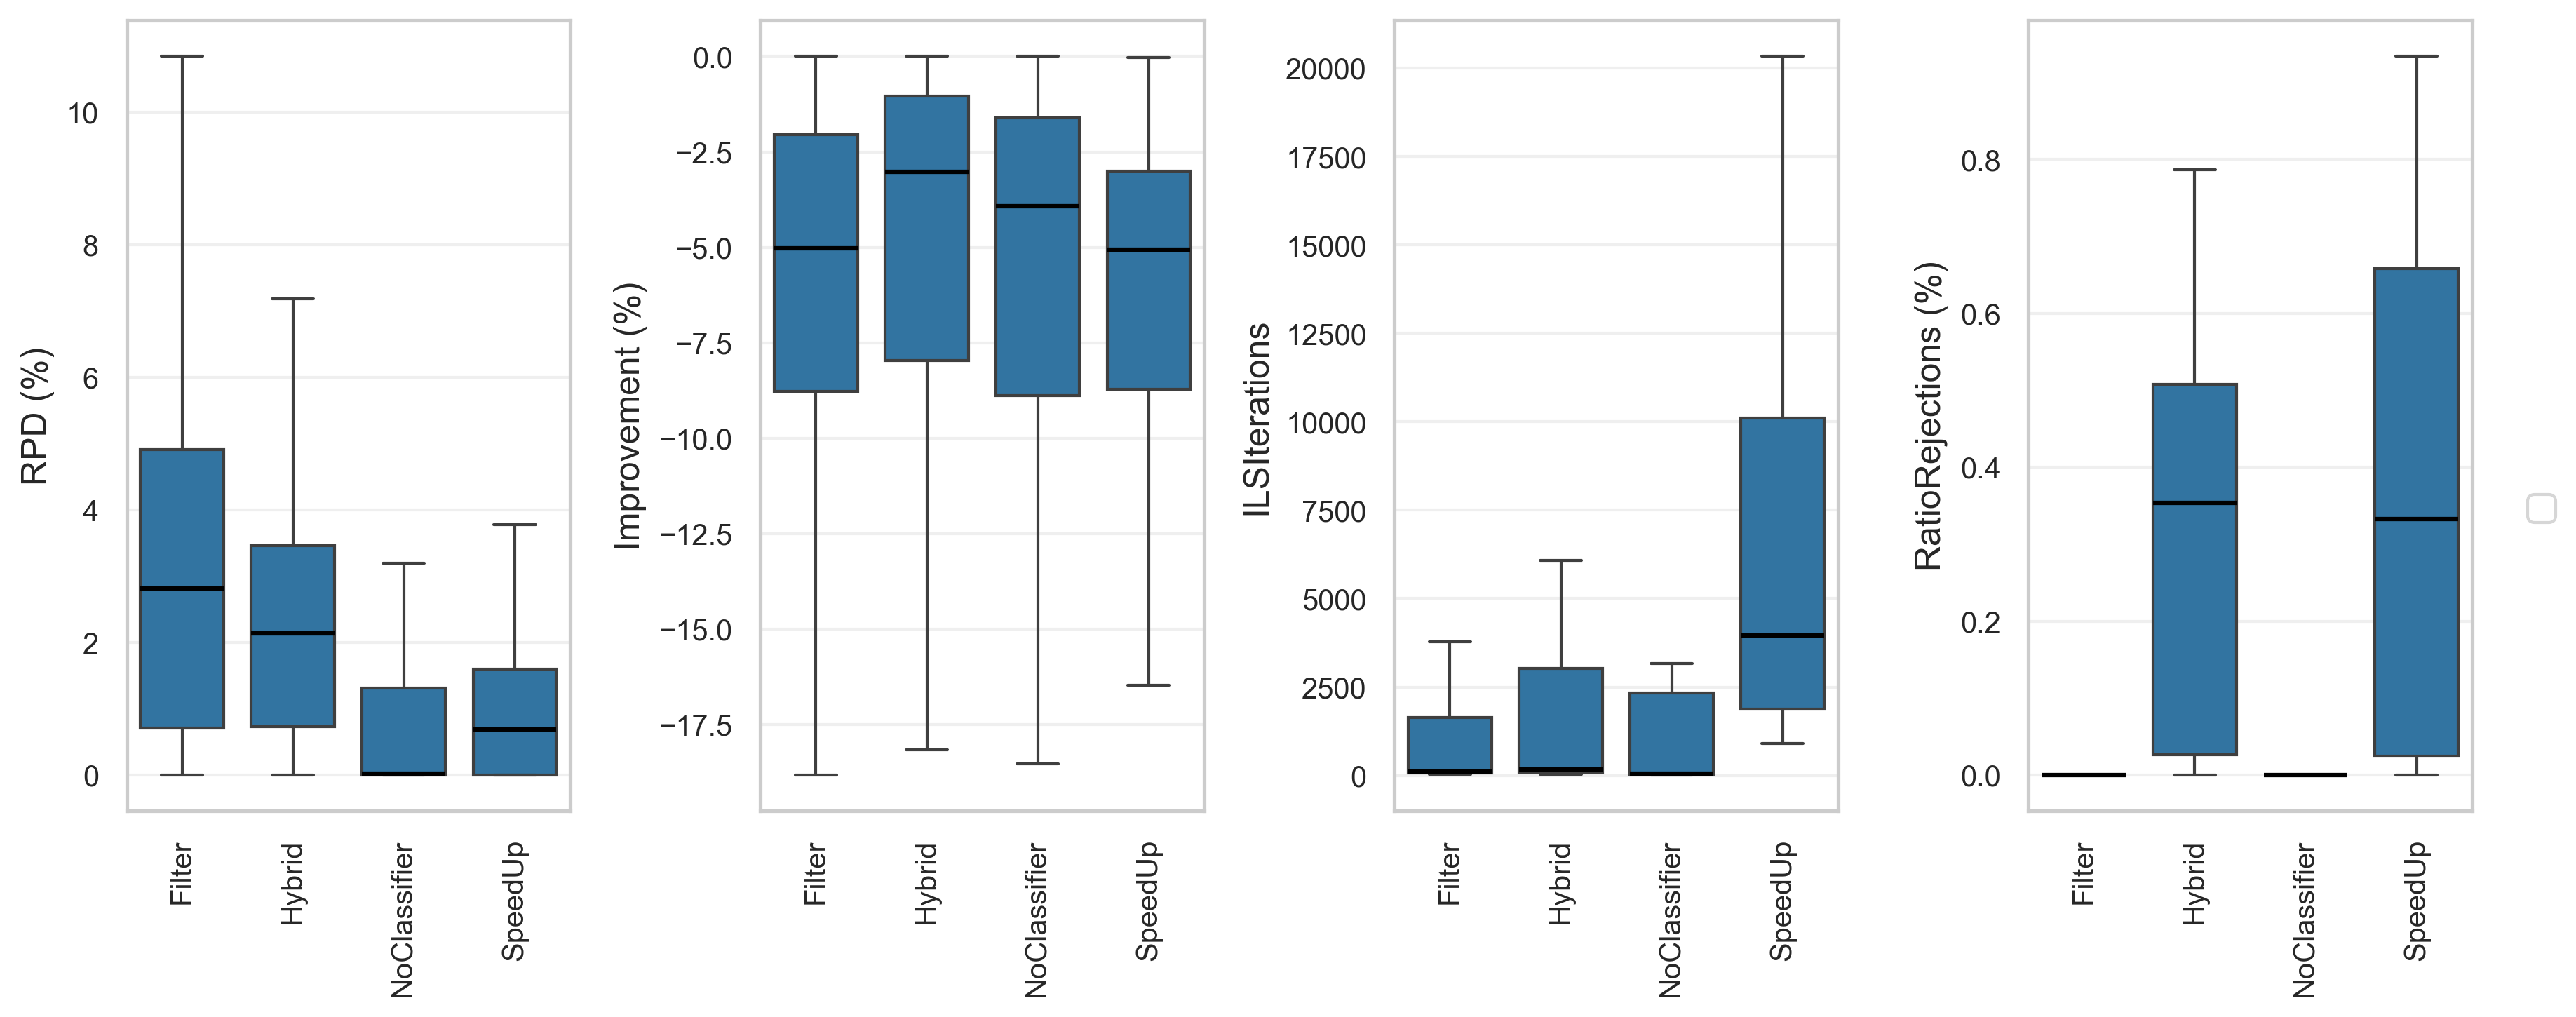
\includegraphics[width =\textwidth]{pictures/final_results/LoadingCheckerType_boxplot_final_results.png}
	\caption{Comparison of all different ILS variants depending the RPD, the average improvement, iterations and rejection rate.}
	\label{fig:boxplots_final_comparison}
\end{figure}
The NoClassifier variant exhibits the lowest median \gls{RPD} and completes the fewest iterations within the time limit.
The SpeedUp variant is the best-performing classifier variant, achieving a low \gls{RPD} and significantly more iterations per
instance, which consequently yields a higher percentage improvement from the constructive to the best solution.
Although the Filter variant achieves a moderate improvement, its overall performance is poor because false negative predictions
lead to worse solutions. The Hybrid variant attains decent \gls{RPD} values. However, its iteration count is quite low
compared to the SpeedUp variant. This behavior was discussed in the previous section, where the specific setup (\gls{CP} check in the inter-neighborhood)
was chosen to differentiate it from the SpeedUp variant. The following Table~\ref{tab:mean_final_results}
summarizes the mean performance indicator values for each variant.
\begin{table}
	\centering
	\small
	\begin{tabular}{lrrrrrr}
		\toprule
		Variant      & RPD  & Iterations & Improvement & RatioRejection & $t_0$ & $C_0$   \\
		\midrule
		Filter       & 3.08 & 2944.36    & -6.18       & 0.00           & 12.65 & 1024.53 \\
		Hybrid       & 2.36 & 3146.44    & -5.51       & 0.31           & 25.70 & 1007.83 \\
		NoClassifier & 0.84 & 2895.44    & -5.61       & 0.00           & 30.74 & 1010.54 \\
		SpeedUp      & 1.07 & 6124.06    & -7.27       & 0.36           & 23.49 & 1014.09 \\
		\bottomrule
	\end{tabular}
	\caption[Comparison of mean results between variants.]{Comparison of mean results between variants. $t_0$ displays the time for the start solution and $C_0$ is the start solution objective.}
	\label{tab:mean_final_results}
\end{table}
It should be noted that the mean number of iterations is considerably higher than the median. Notably, the difference in \gls{RPD}
values between the NoClassifier and SpeedUp variants has decreased. Overall, the rejection ratio is quite low, resulting in
the reversion of only about one third of all iterations. The median values per configuration are presented in
Table~\ref{tab:final_mean_comparison} in the Appendix. Additionally, the visualizations for each classifier variant in the following overview
illustrate the influence of different configurations:
\begin{table}[ht]
	\centering
	\setlength{\tabcolsep}{12pt}
	\begin{tabular}{ccc}
		Filter: Figure~\ref{fig:final_results_filter_variant} & SpeedUp: Figure~\ref{fig:final_results_speedup_variant} & Hybrid: Figure~\ref{fig:final_results_hybrid_variant}
	\end{tabular}
\end{table}
However, the differences between individual models and datasets for each variant are surprisingly small and do not significantly
affect the overall results. Beyond the average statistics, the per-instance results are compared in the following. The best solution
per variant is compared both among the variants and against the \gls{BKS} in Table~\ref{tab:final_best_results_gendreau}. Compared to Table~\ref{tab:bc_results_gendreau},
only heuristic approaches are considered. The publisher of the \gls{BKS}
for the \gendreauDataSetText~dataset is indicated by the lowercase letter in the \gls{BKS} column. In this comparison,
all published studies, using the same loading constraint set $\mathcal{G}$, were taken into account.
\begin{table}[ht]
	\centering
	\small
	\begin{tabular}{L{6cm}lccc}
		\toprule
		                                                                             &       & \multicolumn{3}{c}{Timelimit [sec]}                                                                                                       \\\cmidrule(lr){3-5}
		Author                                                                       & Label & $N \leq 25$                                                     & $25 < N \leq 50$                   & $50 < N$                           \\
		\midrule
		\cite{tarantilis_hybrid_2009}\footcite[cf.][p. 264]{tarantilis_hybrid_2009}  & a     & 1800                                                            & 3600                               & 7200                               \\
		\cite{wang_two_2010} \footcite[cf.][p. 265f.]{wang_two_2010}                 & b     & 1800                                                            & 3600                               & 7200                               \\
		\cite{bortfeldt_hybrid_2012}\footcite[cf.][p. 2253]{bortfeldt_hybrid_2012}   & c     & 180\footnote{Start solution time was excluded from time limit.} & 300\footnotemark[\value{footnote}] & 400\footnotemark[\value{footnote}] \\
		\cite{zhang_evolutionary_2015}\footcite[cf.][p. 28]{zhang_evolutionary_2015} & d     & 900                                                             & 1800                               & 3600                               \\
		This thesis                                                                  & -     & 600                                                             & 600                                & 600                                \\

		\bottomrule
	\end{tabular}
	\caption[Different time limits for \gendreauDataSetText instances from various authors.]
	{Different time limits for \gendreauDataSetText instances from various authors dependent of customer number $N$.}
	\label{tab:timeLimit_comparison}
\end{table}

\begin{table}[ht]
	\centering
	\scriptsize
	\renewcommand{\arraystretch}{1.02}
	\begin{tabular}{@{}llcccccccc@{}}
		\toprule
		                    &                             & \multicolumn{2}{c}{NoClassifier} & \multicolumn{2}{c}{Filter} & \multicolumn{2}{c}{SpeedUp} & \multicolumn{2}{c}{Hybrid}                                                                    \\ \cmidrule(lr){3-4}\cmidrule(lr){5-6}\cmidrule(lr){7-8}\cmidrule(lr){9-10}
		Instance            & BKS                         & $C^*$                            & $\Delta BKS$               & $C^*$                       & $\Delta BKS$               & $C^*$            & $\Delta BKS$ & $C^*$           & $\Delta BKS$ \\
		\midrule
		$\text{E016-03m}^H$ & $\text{301.74}^b$           & \textbf{301.66}                  & -0.03                      & 301.74                      & 0.00                       & 301.74           & 0.00         & 301.74          & 0.00         \\
		$\text{E016-05m}^H$ & $\text{\textbf{334.96}}^a$  & \textbf{334.96}                  & 0.00                       & \textbf{334.96}             & 0.00                       & \textbf{334.96}  & 0.00         & \textbf{334.96} & 0.00         \\
		$\text{E021-04m}^H$ & $\text{\textbf{385.53}}^d$  & 392.25                           & 1.74                       & \textbf{385.53}             & 0.00                       & \textbf{385.53}  & 0.00         & \textbf{385.53} & 0.00         \\
		$\text{E021-06m}^H$ & $\text{437.19}^b$           & \textbf{430.88}                  & -1.44                      & \textbf{430.88}             & -1.44                      & \textbf{430.88}  & -1.44        & \textbf{430.88} & -1.44        \\
		$\text{E022-04g}^H$ & $\text{436.48}^b$           & \textbf{427.68}                  & -2.02                      & 437.27                      & 0.18                       & 437.27           & 0.18         & 437.27          & 0.18         \\
		$\text{E022-06m}^H$ & $\text{\textbf{498.16}}^c$  & \textbf{498.16}                  & 0.00                       & \textbf{498.16}             & 0.00                       & \textbf{498.16}  & 0.00         & \textbf{498.16} & 0.00         \\
		$\text{E023-03g}^L$ & $\text{767.46}^b$           & \textbf{757.88}                  & -1.25                      & 774.74                      & 0.95                       & 774.74           & 0.95         & 774.74          & 0.95         \\
		$\text{E023-05s}^L$ & $\text{803.98}^b$           & \textbf{800.98}                  & -0.37                      & 803.48                      & -0.06                      & 803.48           & -0.06        & 803.48          & -0.06        \\
		$\text{E026-08m}^H$ & $\text{\textbf{630.13}}^b$  & \textbf{630.13}                  & 0.00                       & 643.61                      & 2.14                       & 643.61           & 2.14         & 643.61          & 2.14         \\
		$\text{E030-03g}^L$ & $\text{820.35}^c$           & 834.25                           & 1.69                       & 820.78                      & 0.05                       & \textbf{818.54}  & -0.22        & 831.43          & 1.35         \\
		$\text{E030-04s}^L$ & $\text{768.25}^b$           & 779.33                           & 1.44                       & 786.03                      & 2.31                       & \textbf{764.58}  & -0.48        & 782.64          & 1.87         \\
		$\text{E031-09h}^H$ & $\text{\textbf{610.23}}^b$  & 614.60                           & 0.72                       & \textbf{610.23}             & 0.00                       & \textbf{610.23}  & 0.00         & 614.23          & 0.66         \\
		$\text{E033-03n}^L$ & $\text{2645.95}^c$          & 2627.28                          & -0.71                      & 2652.72                     & 0.26                       & \textbf{2605.58} & -1.53        & 2641.27         & -0.18        \\
		$\text{E033-04g}^L$ & $\text{\textbf{1363.04}}^d$ & 1374.68                          & 0.85                       & 1434.76                     & 5.26                       & 1417.98          & 4.03         & 1448.18         & 6.25         \\
		$\text{E033-05s}^L$ & $\text{1338.22}^d$          & 1360.96                          & 1.70                       & 1344.54                     & 0.47                       & \textbf{1331.57} & -0.50        & 1343.12         & 0.37         \\
		$\text{E036-11h}^H$ & $\text{\textbf{698.61}}^a$  & 703.35                           & 0.68                       & \textbf{698.61}             & 0.00                       & \textbf{698.61}  & 0.00         & \textbf{698.61} & 0.00         \\
		$\text{E041-14h}^H$ & $\text{\textbf{866.4}}^c$   & 871.63                           & 0.60                       & \textbf{866.40}             & 0.00                       & \textbf{866.40}  & 0.00         & 871.63          & 0.60         \\
		$\text{E045-04f}^L$ & $\text{\textbf{1201.85}}^d$ & 1223.24                          & 1.78                       & 1216.45                     & 1.21                       & 1210.55          & 0.72         & 1218.15         & 1.36         \\
		$\text{E051-05e}^L$ & $\text{\textbf{741.64}}^d$  & 745.05                           & 0.46                       & 765.95                      & 3.28                       & 742.16           & 0.07         & 758.11          & 2.22         \\
		$\text{E072-04f}^L$ & $\text{\textbf{570.17}}^d$  & 598.93                           & 5.04                       & 603.84                      & 5.91                       & 600.74           & 5.36         & 619.27          & 8.61         \\
		$\text{E076-07s}^L$ & $\text{\textbf{1044.26}}^d$ & 1102.90                          & 5.62                       & 1098.45                     & 5.19                       & 1071.07          & 2.57         & 1093.32         & 4.70         \\
		$\text{E076-08s}^L$ & $\text{\textbf{1133.06}}^d$ & 1183.29                          & 4.43                       & 1173.34                     & 3.55                       & 1151.58          & 1.63         & 1172.79         & 3.51         \\
		$\text{E076-10e}^L$ & $\text{\textbf{1084.17}}^d$ & 1143.31                          & 5.45                       & 1142.31                     & 5.36                       & 1108.80          & 2.27         & 1133.43         & 4.54         \\
		$\text{E076-14s}^H$ & $\text{\textbf{1092.46}}^d$ & 1142.99                          & 4.63                       & 1134.57                     & 3.86                       & 1105.02          & 1.15         & 1131.63         & 3.59         \\
		$\text{E101-08e}^L$ & $\text{\textbf{1338.35}}^d$ & 1384.10                          & 3.42                       & 1389.00                     & 3.78                       & 1364.01          & 1.92         & 1382.53         & 3.30         \\
		$\text{E101-10c}^L$ & $\text{\textbf{1530.05}}^d$ & 1653.41                          & 8.06                       & 1628.43                     & 6.43                       & 1600.59          & 4.61         & 1652.37         & 7.99         \\
		$\text{E101-14s}^L$ & $\text{\textbf{1472.11}}^d$ & 1516.77                          & 3.03                       & 1556.54                     & 5.74                       & 1505.07          & 2.24         & 1544.81         & 4.94         \\\midrule
		mean                & 922.77                      & 942.02                           & 1.69                       & 945.68                      & 2.02                       & 932.72           & 0.95         & 946.22          & 2.13         \\
		\bottomrule
	\end{tabular}
	\caption[Results of all four variants in comparison to best known heuristic solutions for \gendreauDataSet.]
	{Results of all four variants in comparison to best known heuristic solutions for \gendreauDataSet. Bold font indicates the
		minimum costs including the BKS. $\Delta BKS$ is the procentual difference to the BKS}
	\label{tab:final_best_results_gendreau}
\end{table}

Out of the 27 \gls{BKS} reported in the literature, 9 were improved using the presented algorithm. Among these,
both the SpeedUp and NoClassifier variants individually achieved four improvements each. In general, the SpeedUp variant performs
better on medium- to large-sized instances compared to the NoClassifier variant. For these larger instances, the higher number of
iterations becomes increasingly valuable, allowing more extensive search and solution refinement.
Overall, the SpeedUp variant achieves the lowest mean deviation from the \gls{BKS} at 0.95\%, followed by NoClassifier with 1.69\%,
representing the second-best result. The Filter variant performs slightly better than the Hybrid variant in this comparison. The
strong performance of the proposed algorithm is further emphasized by the fact that the time limits used to obtain the \gls{BKS}
in previous studies were, for most authors, up to 12 times longer than those used in this work (see Table~\ref{tab:timeLimit_comparison}).
The mean costs per run for each variant are summarized in Table~\ref{tab:final_mean_comparison}, confirming that the SpeedUp
and NoClassifier variants yield the best results. Consistently, the SpeedUp variant shows a slight advantage on medium- and large-sized
instances, whereas the Filter and Hybrid variants demonstrate weaker average performance. In the next chapter, the presented
algorithm with its variants is applied to the \krebsADataSetText dataset.